% !TEX TS-program = pdflatex
% !TEX encoding = UTF-8 Unicode

% This is a simple template for a LaTeX document using the "article" class.
% See "book", "report", "letter" for other types of document.

\documentclass[11pt]{article} % use larger type; default would be 10pt

\usepackage[utf8]{inputenc} % set input encoding (not needed with XeLaTeX)
\usepackage[english, french]{babel}	% change the language to french
\usepackage[light,condensed,math]{iwona}
\usepackage[T1]{fontenc}
%%% Examples of Article customizations
% These packages are optional, depending whether you want the features they provide.
% See the LaTeX Companion or other references for full information.

%%% PAGE DIMENSIONS
\usepackage{geometry} % to change the page dimensions
\geometry{a4paper} % or letterpaper (US) or a5paper or....
\geometry{margin=0.8in} % for example, change the margins to 2 inches all round
% \geometry{landscape} % set up the page for landscape
%   read geometry.pdf for detailed page layout information

\usepackage{graphicx} % support the \includegraphics command and options
\graphicspath{ {images/} }
\usepackage{subfig}	% pour afficher les sous-graphiques cote a cote
% \usepackage{caption}
% \usepackage{subcaption}	% pour afficher les sous-graphiques cote a cote
\usepackage{fixltx2e}	% Pour les trucs de math
\usepackage{mathtools}	
\usepackage{newunicodechar}
\usepackage{gensymb}
\usepackage{csquotes}	%Pour les guillements
\usepackage{textgreek}		% pour les lettres grecques
\usepackage{amssymb }
\usepackage{xcolor}	% pour les couleurs

% \usepackage[parfill]{parskip} % Activate to begin paragraphs with an empty line rather than an indent

%%% PACKAGES
\usepackage{booktabs} % for much better looking tables
\usepackage{array} % for better arrays (eg matrices) in maths
\usepackage{paralist} % very flexible & customisable lists (eg. enumerate/itemize, etc.)
\usepackage{verbatim} % adds environment for commenting out blocks of text & for better verbatim
\usepackage{subfig} % make it possible to include more than one captioned figure/table in a single float
% These packages are all incorporated in the memoir class to one degree or another...

%%% HEADERS & FOOTERS
\usepackage{fancyhdr} % This should be set AFTER setting up the page geometry
\pagestyle{fancy} % options: empty , plain , fancy
\renewcommand{\headrulewidth}{0pt} % customise the layout...
\lhead{}\chead{}\rhead{}
\lfoot{}\cfoot{\thepage}\rfoot{}

%%% SECTION TITLE APPEARANCE
\usepackage{sectsty}
\allsectionsfont{\sffamily\mdseries\upshape} % (See the fntguide.pdf for font help)
% (This matches ConTeXt defaults)

%%% ToC (table of contents) APPEARANCE
\usepackage[nottoc,notlof,notlot]{tocbibind} % Put the bibliography in the ToC
\usepackage[titles,subfigure]{tocloft} % Alter the style of the Table of Contents
\renewcommand{\cftsecfont}{\rmfamily\mdseries\upshape}
\renewcommand{\cftsecpagefont}{\rmfamily\mdseries\upshape} % No bold!

%%% END Article customizations

%%% The "real" document content comes below...

\title{PROJET \\ Simulation thermique d'une ailette d'un dissipateur de chaleur}
\author{Roussel Desmond Nzoyem Ngueguin}
%\date{} % Activate to display a given date or no date (if empty),
         % otherwise the current date is printed 

\begin{document}
\begin{titlepage}

\centering
\vspace*{\fill}
\large \bf SIMULATION THERMIQUE D'UNE AILETTE D'UN DISSIPATEUR DE CHALEUR \\
\large \rm Roussel Desmond Nzoyem Ngueguin \\
\today \rm
\vspace*{\fill}

%\maketitle
%\thispagestyle{empty}	% pour ne rien afficher en bas de la premiere page

\end{titlepage}
%\newpage

\clearpage
\pagenumbering{arabic}	%Pour commencer le comptage des pages a 1

\section*{Introduction}

Le programme écrit permet de visualiser le comportement du dispositif de refroidissement d’un microprocesseur. Le dispositif étudié est constitué d’un ventilateur et d’un dissipateur de chaleur rattaché au processeur \textbf{(figure 1)}. 
	
\begin{figure}[!htb]
	\centering
	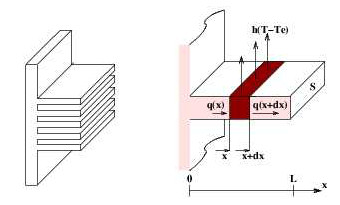
\includegraphics[scale=0.7]{fig_1}
	\caption{Modelisation d'une ailette du dissipateur}
\end{figure}

L’équation de la chaleur sur une ailette supposé suffisamment mince pour que la température en un point donné ne dépende que sa position x a un instant t donné est:
\begin{equation}
	\rho C_{p}\frac{\partial T} {\partial t} - \kappa \frac{\partial ^{2}T}{\partial x^{2}} + \frac{h_{c}p}{S} (T-T_{e}) = 0
\end{equation}
\par Avec ρ la densité, C\textsubscript p la chaleur spécifique a pression constante, κ la conductivité thermique, h\textsubscript c le coefficient de transfert de chaleur surfacique, T\textsubscript e la température ambiante, S = L\textsubscript yL\textsubscript z l'aire d'une section transversale et p = 2(L\textsubscript x + L\textsubscript y) le périmètre d'une section transversale. L\textsubscript x, L\textsubscript y, et L\textsubscript z étant les longueurs de l’ailette. En x=0, le flux dégagé par le processeur vaut \textPhi \textsubscript p. En x=L\textsubscript x, le flux est supposé négligeable par rapport au flux apporté par la section longitudinale.

\par Après avoir décrit la structure du programme C++, nous effectuerons des simulations sur une des ailettes du dissipateur.


\section{Description de la structure du programme }

Une classe \textquote{Stationnaire} est définie pour traiter le modèle stationnaire, et une classe \textquote{Instationnaire} (dérivée de \textquote{Stationnaire}) est définie pour traiter le modèle instationnaire. Le point d’entrée du programme se charge de lire le fichier de configuration et de créer les objets qui vont contenir le problème et le résoudre.

	\subsection{Exécution du programme}
Plusieurs fichiers sont nécessaires à l’exécution du programme :
\begin{itemize}
	\item \textbf{Les fichiers headers} (stationnaire.hpp et instationnaire.hpp) : ils contiennent les déclarations des classes Stationnaire et Instationnaire ;
	\item \textbf{Les fichiers sources} (cooling.cpp, stationnaire.cpp, et instationnaire.cpp) : ils contiennent les définitions des classes. Le fichier cooling.cpp contient la fonction main() qui lit les paramètres. Avec ces données, elle crée un nouveau problème (un objet), qui va "se résoudre". Puis elle supprime l’objet créé.
	\item \textbf{Les commandes gnuplot} (gnuplot\textunderscore command\textunderscore *.dat) : ces fichiers contiennent les commandes à exécuter par le programme préinstallé "gnuplot" pour visualiser les solutions 1D.
	\item \textbf{Les fichiers de configuration} (simu\textunderscore 0.cfg, simu\textunderscore 1.cfg, …, simu\textunderscore 11.cfg) : localisés dans le répertoire "config\textunderscore files", ils contiennent les paramètres physiques, géométriques, et de simulation du problème. Ces 17 paramètres peuvent être lus dans n’importe quel ordre, à condition de bien les nommer (l’unité de longueur étant le mètre).
\end{itemize}
\par Une fois chacun de ces fichiers dans le répertoire approprié, l’exécution de la commande :
{
\color{blue}
\begin{verbatim}
	g++ cooling.cpp stationnaire.cpp instationnaire.cpp -o cooling && ./cooling simu_1.cfg
\end{verbatim}
}
\noindent devrait lancer la simulation 1. Le programme s’assurera de la résolution du problème, de l’écriture des solutions dans des fichiers .csv et .vtk, puis de l’affichage 1D de la solution correspondant au problème (avec "gnuplot").
	
	\subsection{Fonctions majeures du programme}
	
Toutes les fonctions du programmes (hormis main())sont des méthodes définies dans les fichiers stationnaire.cpp et instationnaire.cpp. Parmi elles, les plus importantes sont les suivantes :
\begin{itemize}
	\item\textbf{void Stationnaire::factoLU() }: effectue la factorisation LU de la matrice A
	\item\textbf{void Stationnaire::descenteRemontee() }: résout le problème AX = F , avec A = LU
	\item\textbf{void Stationnaire::searchInterval() }: localise les points x\textsubscript{i00} dans le maillage 1D, nécessaire pour effectuer l’interpolation linéaire
	\item\textbf{void Stationnaire::interpolationLineaire() }: calcule l’interpolant linéaire aux différents points x\textsubscript{i00}
	\item\textbf{bool Stationnaire::ecriture3D(int indice\textunderscore temps, bool flux\textunderscore de\textunderscore chaleur\textunderscore constant) }: Permet d’écrire un fichier .vtk dans le répertoire "paraview\textunderscore data" en vue de la visualisation 3D. Elle prend en entrée l’indice de l’itération à laquelle la solution a été calculé (compris entre 0 et N pour les cas instationnaires, et qui vaut -1 dans le cas stationnaire). Ce numéro sera nécessaire pour nommer le fichier créé. La fonction prend aussi en entrée un booléen disant si on traire le problème instationnaire au scénario 1 (=true) ou au scénario 2 (=false). Elle nous retourne un booléen disant si l’écriture a été un succès ou pas.
	\item\textbf{void Stationnaire::solve() }: fonction virtuelle qui remplit la matrice A, appelle les fonction nécessaires pour résoudre le problème, et écrit la solution stationnaire dans le fichier .vtk
	\item\textbf{void Stationnaire::solveAnalytiqueStationnaire() }: calcule la solution stationnaire exacte
	\item\textbf{void Stationnaire::displayPlot() const }: fonction virtuelle qui écrit la solution dans le fichier .csv et effectue la visualisation 1D du problème stationnaire
	\item\textbf{void Instationnaire::solve() }: fonction qui surcharge la méthode solve() du cas stationnaire, rempli la matrice A, appelle les fonction nécessaires pour résoudre le probelme, et écris les solution instationnaire à diverses itérations dans les fichiers .vtk
	\item\textbf{void Instationnaire::displayPlot() const }: surcharge la fonction displayPlot() pour écrire dans le fichier .csv, et puis affiche ces solutions (aux différents instants, ou à différentes positions, en fonction du scénario traité)
\end{itemize}
	
	\subsection{Strucure UML}
	
	Les autres fonctions et attributs sont representés dans le diagramme de classe UML \textbf{(figure 2)}.
		\begin{figure}[!htb]
			\centering
			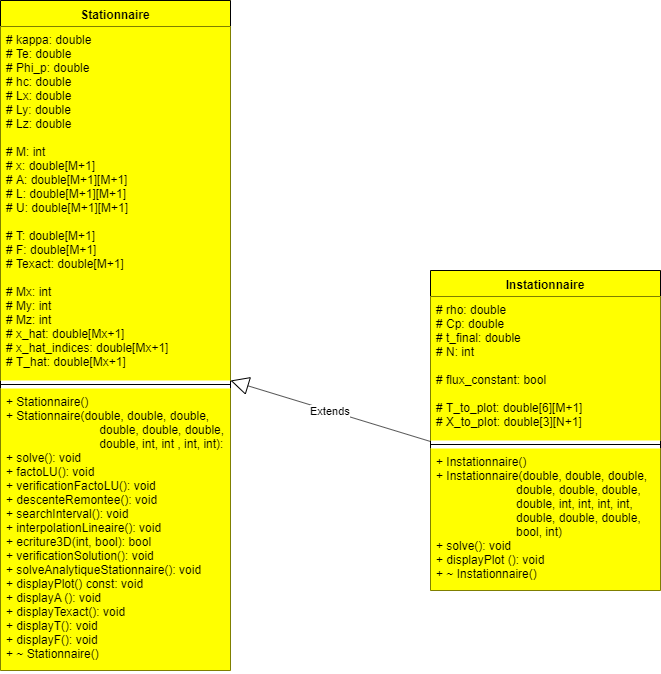
\includegraphics[height=12cm]{fig_2}
			\caption{Digramme de classes du programme}
		\end{figure}
	
	\subsection{Données generées}
	
Les donnes générées sont les fichiers .csv et .vtk pour visualiser respectivement les solutions 1D et 3D. Les fichiers .csv se trouvent dans le répertoire courant (celui contenant le fichier cooling.cpp), alors que les fichiers. vtk sont créer dans le répertoire "paraview\textunderscore data".
\begin{itemize}
	\item\textbf{data\textunderscore stationnaire.csv} : données pour la visualisation 1D de la solution stationnaire calculée et de la solution analytique exacte
	\item\textbf{data\textunderscore instationnaire\textunderscore const.csv} : données pour la visualisation 1D de la température du modèle instationnaire à flux constant (Scenario 1) à 6 instants distinct (t=15s, t=30s, t=60s, t=90s, t=150s, et t=210s)
	\item\textbf{data\textunderscore instationnaire\textunderscore non\textunderscore const.csv} : données pour la visualisation de l’évolution de la température du modèle instationnaire avec activation et désactivation du flux de chaleur venant du processeur toute les 30 secondes (Scenario 2) en 3 points donnés (x=0, x=M/2, et x=M)
	\item\textbf{stationnaire.vtk}: données du modèle stationnaire pour la visualisation 3D avec Paraview
	\item\textbf{instationnaire\textunderscore constant.*.vtk}: données du modèle instationnaire au scénario 1 pour la visualisation 3D avec Paraview
	\item\textbf{instationnaire\textunderscore non\textunderscore constant.*.vtk}: données du modèle instationnaire au scénario 2 pour la visualisation 3D avec Paraview
\end{itemize}

\section{Simulations }

	\subsection{Vérification du code de calcul}

	
		\subsubsection{Cas Stationnaire}
\par On utilise les fichiers de configuration simu\textunderscore0.cfg et simu\textunderscore1.cfg pour visualiser les températures de l’ailette en 1D respectivement pour M = 10 et M=10000. M étant la taille du maillage utilisé pour la discrétisation du problème.
			\begin{figure}[!htb]
				\centering
				\subfloat[M = 10]{{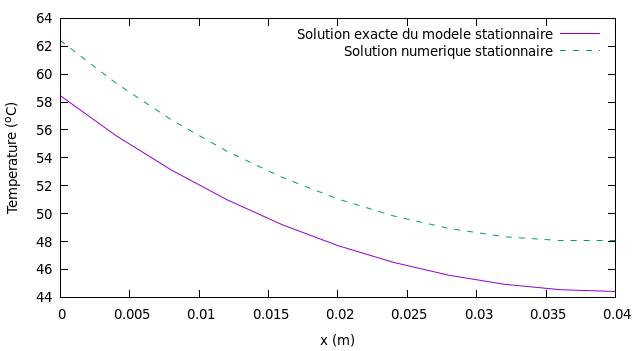
\includegraphics[width=7.5cm]{fig_3} }}%
				\qquad
				\subfloat[M = 10000]{{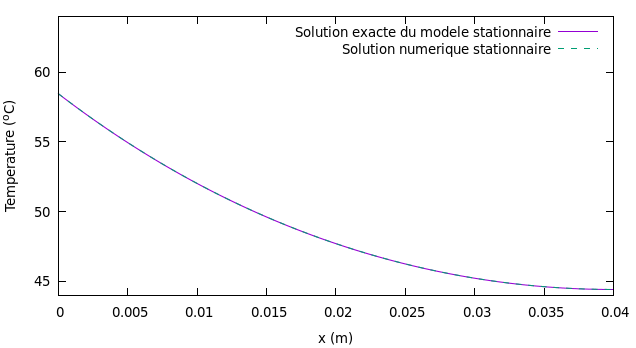
\includegraphics[width=7.5cm]{fig_4} }}%
				\caption{Température dans le modele stationnaire}%
				\label{fig:conv_stat}%
			\end{figure}
\par On constate que la solution calculée par résolution du système linéaire est correcte. Plus le nombre de points de notre maillage est grand, plus les calculs sont précis, et ainsi la solution calculée se rapproche de la solution analytique trouvée a la main.
		\subsubsection{Cas Instationnaire}

			
			\begin{center}
				\textbf{Scenario 1: Flux constant}
			\end{center}
\par Nous utilisons ici le fichier de configuration simu\textunderscore2.cfg
			\begin{figure}[!htb]
				\centering
				\subfloat[Modele stationnaire]{{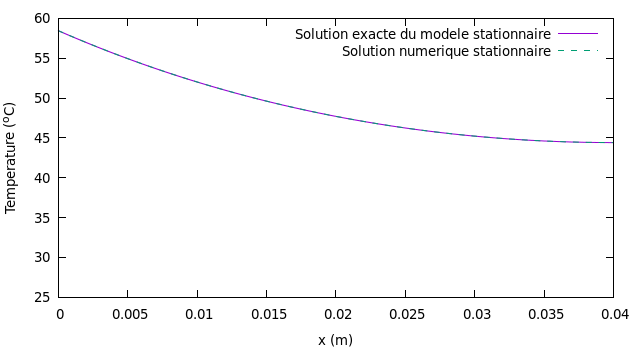
\includegraphics[width=7.5cm]{fig_5} }}%
				\qquad
				\subfloat[Solution iterative du modele instationnaire]{{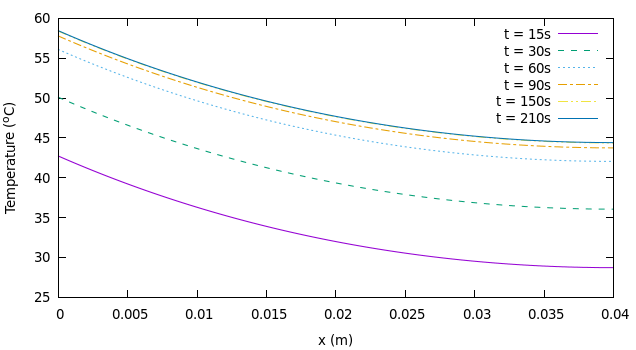
\includegraphics[width=7.5cm]{fig_6} }}%
				\caption{Convergence pour le modele instationnaire vers la solution du modele stationnaire}%
				\label{fig:conv_instat}%
			\end{figure}
\par En 1D, nous pouvons voir que la solution du modèle instationnaire dessiné à différents instants de la simulation se rapproche de la solution du modèle stationnaire \textbf{(figure 4)} .

			\begin{figure}[!htb]
				\centering
				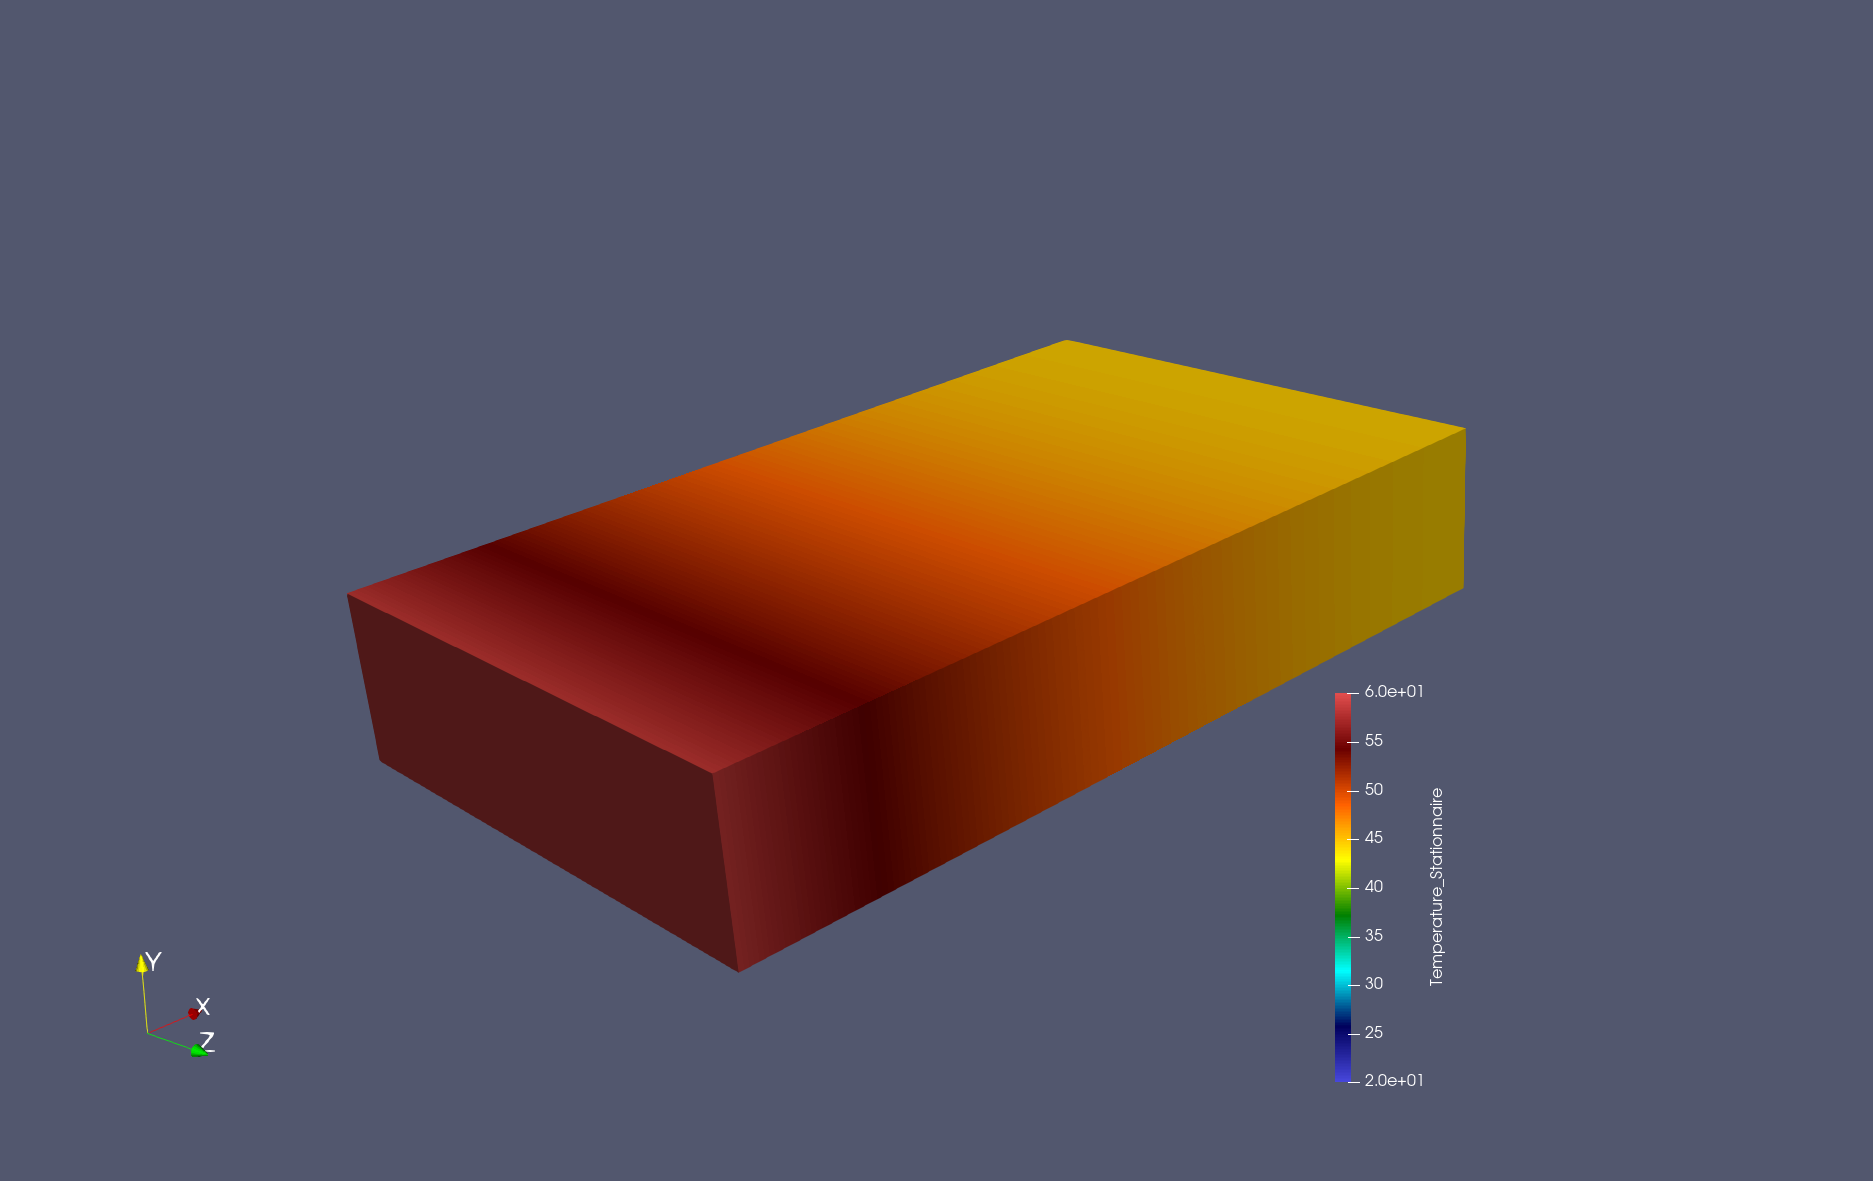
\includegraphics[scale=0.1]{fig_7}
				\caption{Visualisation 3D de la solution du modele stationnaire}	
			%\end{figure}
			%\begin{figure}[!htb]
				\centering
				\subfloat[t = 0s]{{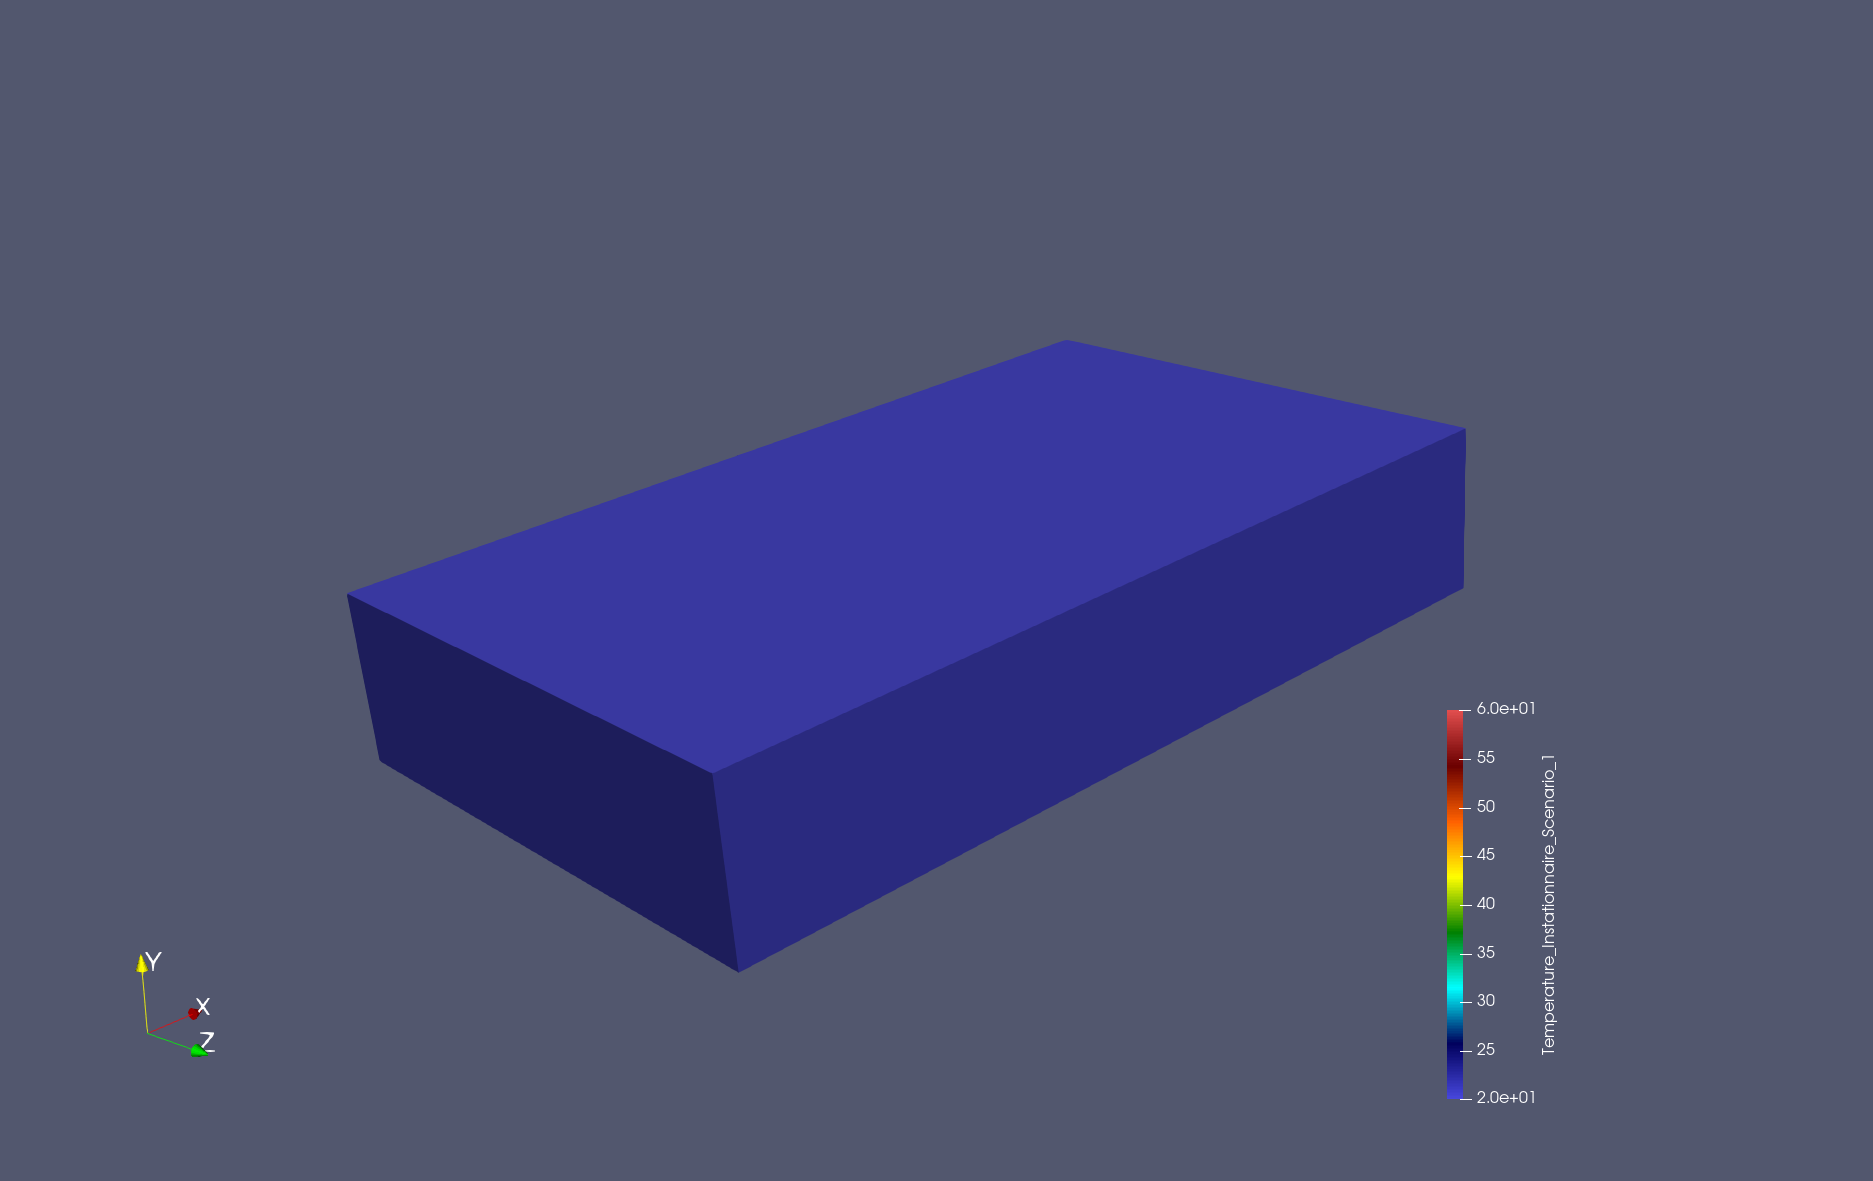
\includegraphics[width=7.5cm]{fig_8} }}%
				\qquad
				\subfloat[t = 30s]{{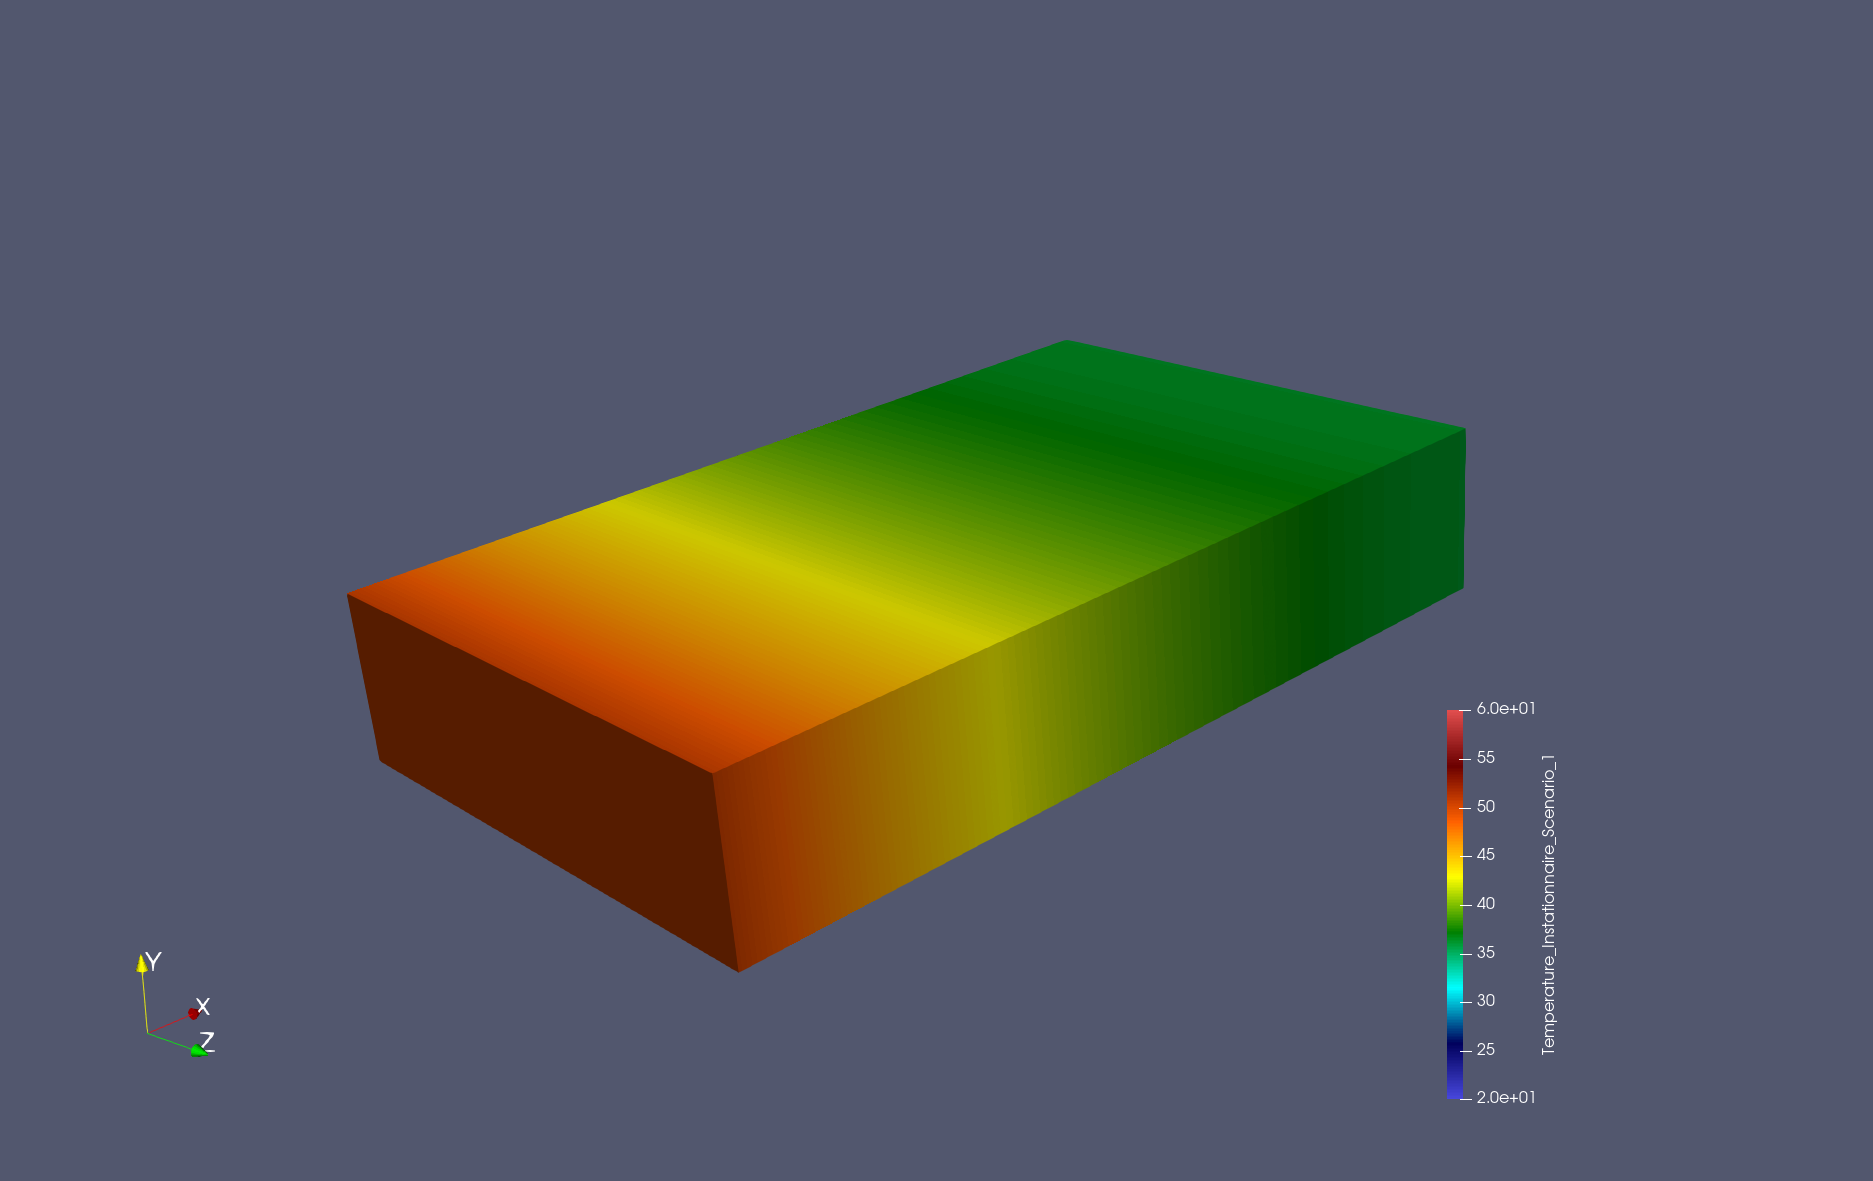
\includegraphics[width=7.5cm]{fig_9} }}%
				\qquad
				\subfloat[t = 90s]{{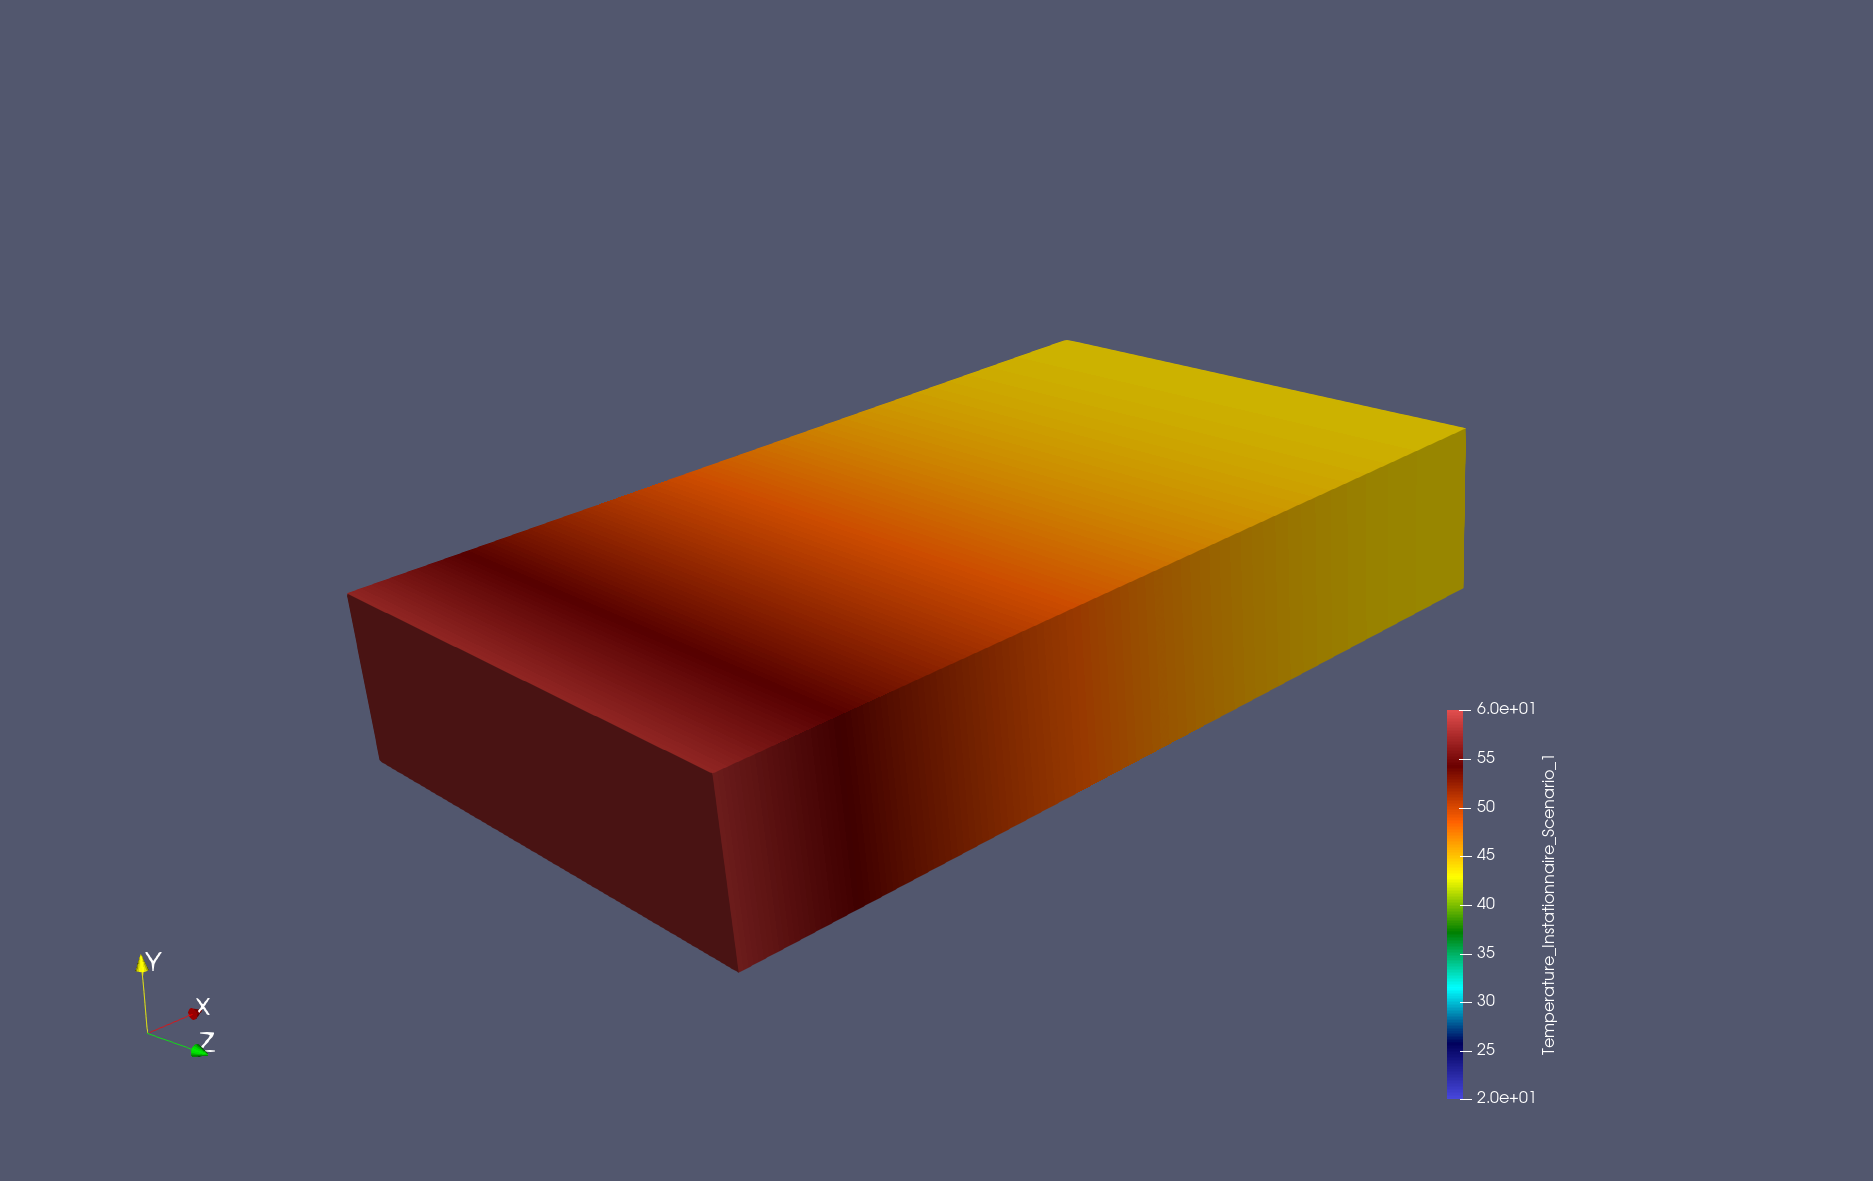
\includegraphics[width=7.5cm]{fig_10} }}%
				\qquad
				\subfloat[t = 300s]{{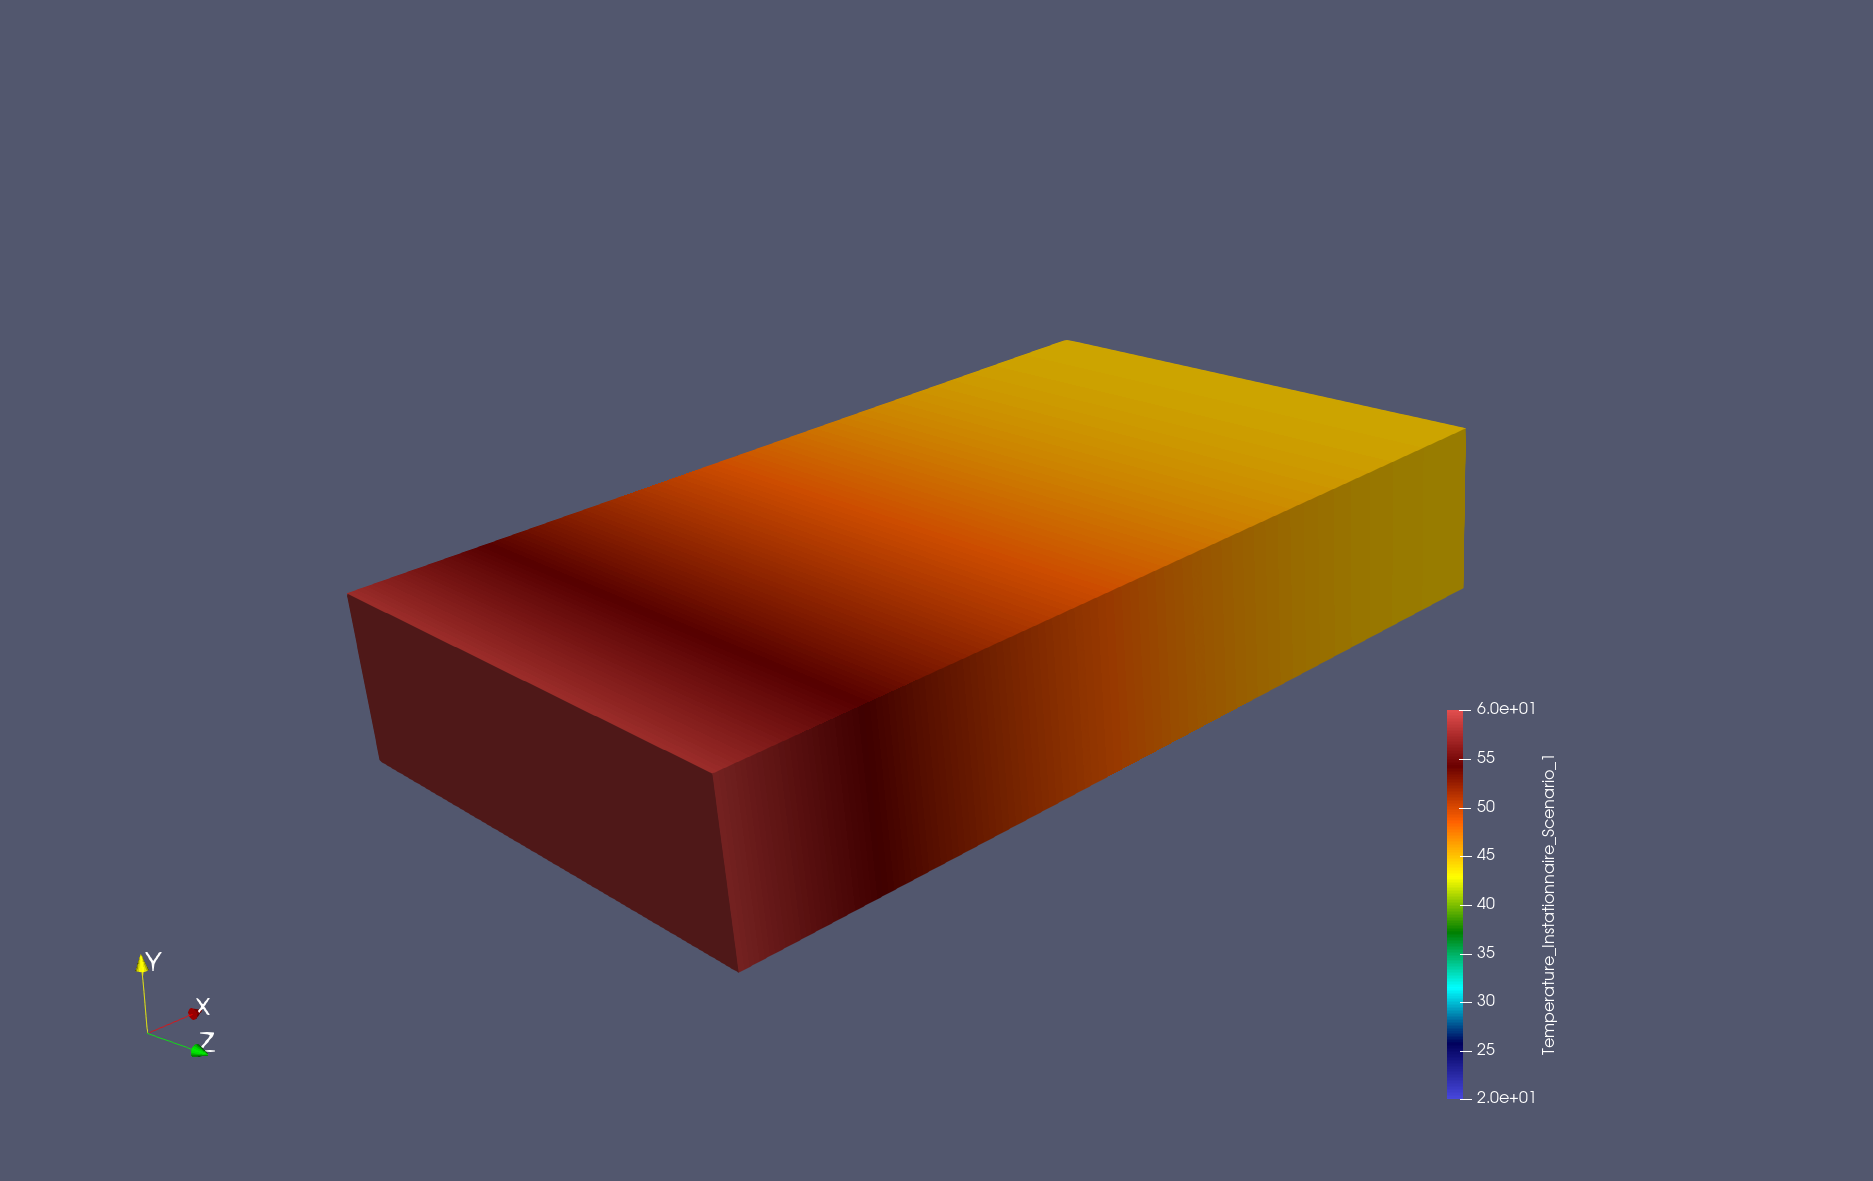
\includegraphics[width=7.5cm]{fig_11} }}%
				\caption{Visualisation 3D de la convergence de la solution du modele instationnaire avec flux constant}%
				\label{fig:conv_instat}%
			\end{figure}
\par En 3D avec Paraview, on observe le meme résultat lorsqu’on observe l’évolution de la température sur l’ailette \textbf{(figures 5 et 6)}.
			\begin{center}
				\textbf{Scenario 2: Flux activé et desactivé toutes les 30 secondes}
			\end{center}
\par Les hypothèses du scénario 2 diffèrent grandement de celles du modèle stationnaire. En effet, on suppose (implicitement) le flux de chaleur émis par le processeur constant pour le modèle stationnaire. La solution dans le scénario 2 ne converge donc pas forcément vers la solution du modèle stationnaire. Mais elle s’y rapproche néanmoins dans certaines circonstances (quoique lentement), en particulier lorsque le ventilateur est éteint, comme nous le montrerons par la suite.
	
	\subsection{Longueur Lx variable}


		\begin{center}
			\textbf{Scenario 1: Flux constant}
		\end{center}
\par Pour trois longueurs L\textsubscript x différentes (40mm, 80mm, 200mm), visualisons le resultat en 1D puis en 3D. Les fichiers de configuration simu\textunderscore4.cfg, simu\textunderscore5.cfg, et simu\textunderscore6.cfg permettent de réaliser ces simulations \textbf{(figures 7, 8, et 9)}. 
			\begin{figure}[!htb]
				\centering
				\subfloat[Evolution de la température]{{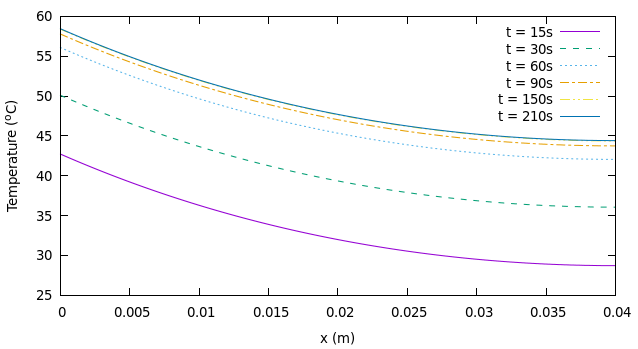
\includegraphics[width=7.5cm]{fig_13} }}%
				\qquad
				\subfloat[Température finale (à t = 300s)]{{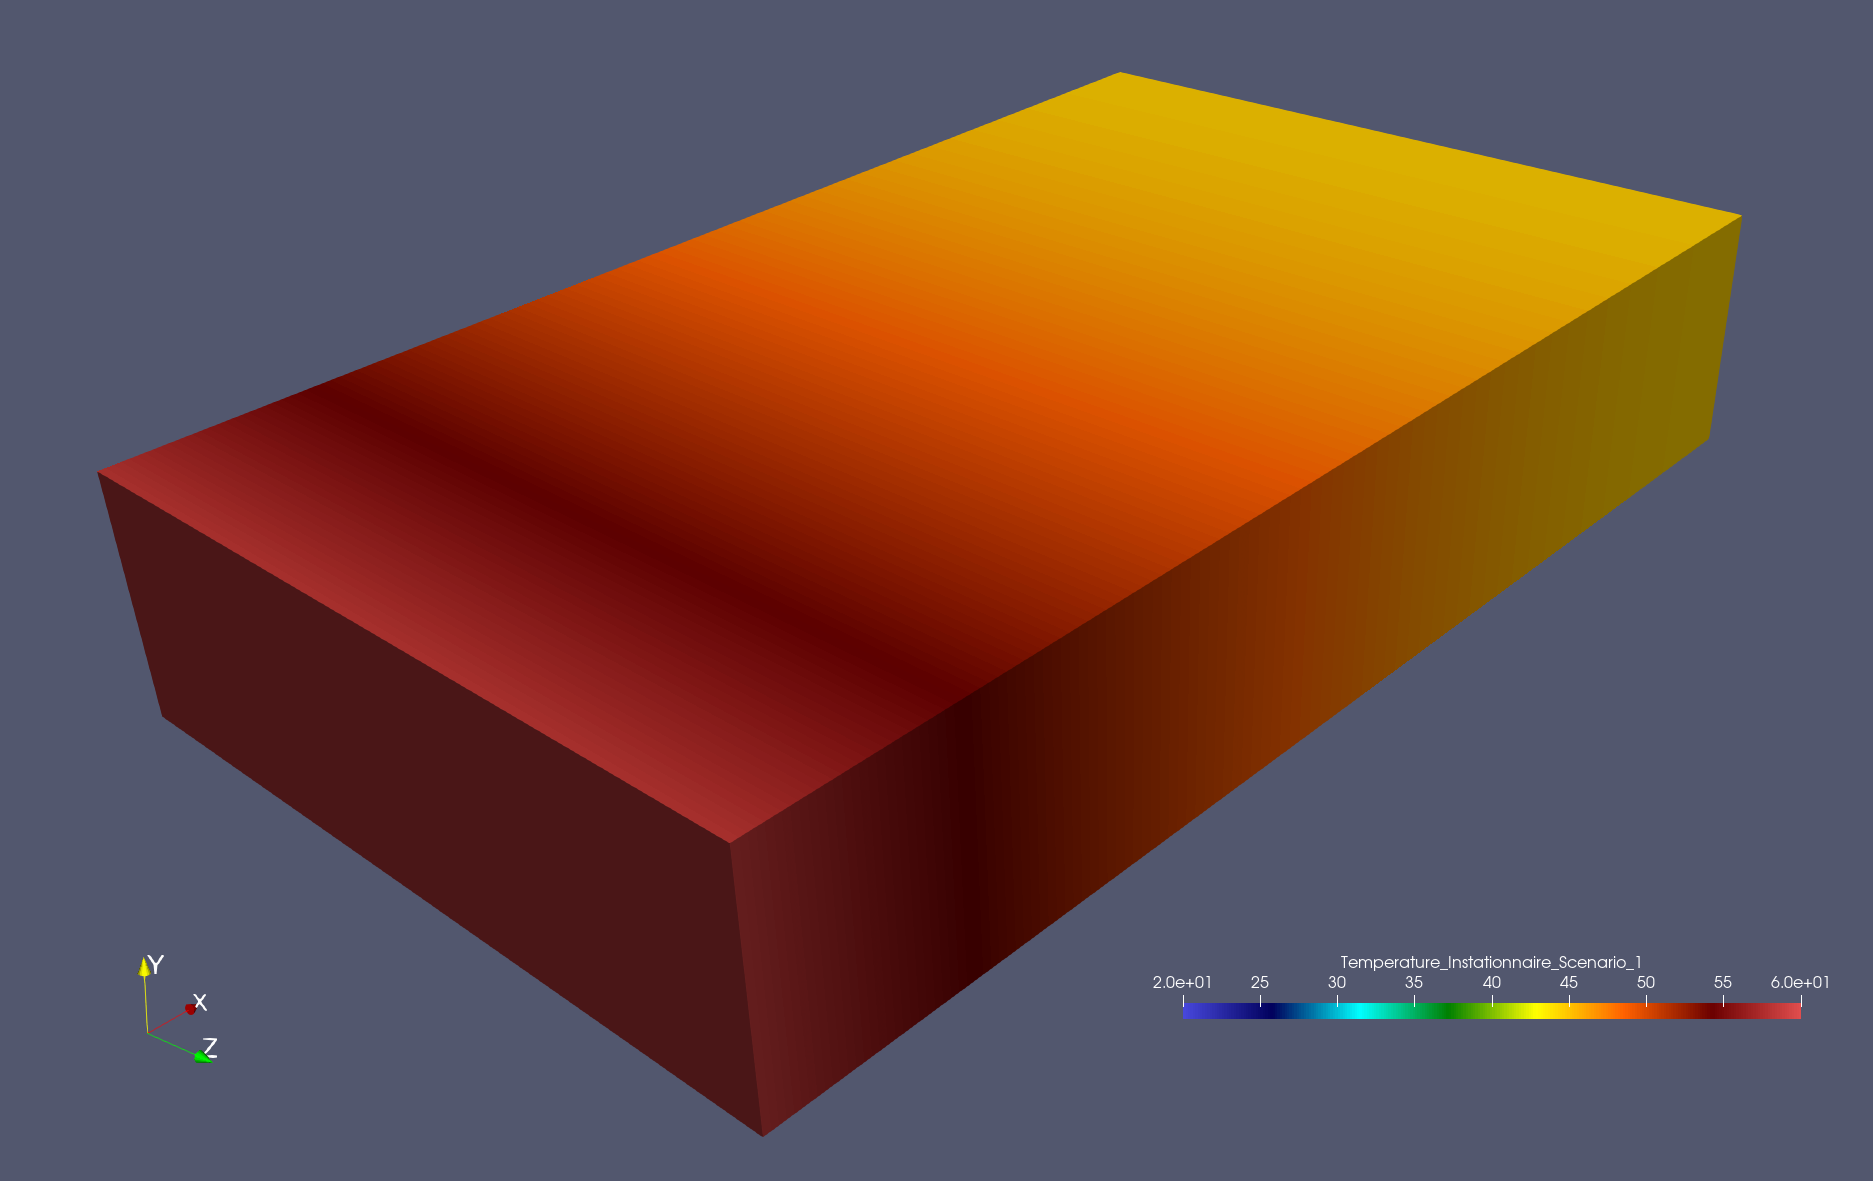
\includegraphics[width=7.5cm]{fig_14} }}%
				\caption{Scénario 1 - Lx = 40 mm}%
			%\end{figure}

			%\begin{figure}[!htb]
				\centering
				\subfloat[Evolution de la température]{{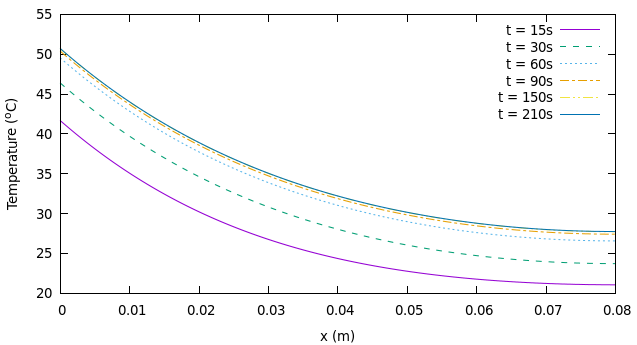
\includegraphics[width=7.5cm]{fig_15} }}%
				\qquad
				\subfloat[Température finale (à t = 300s)]{{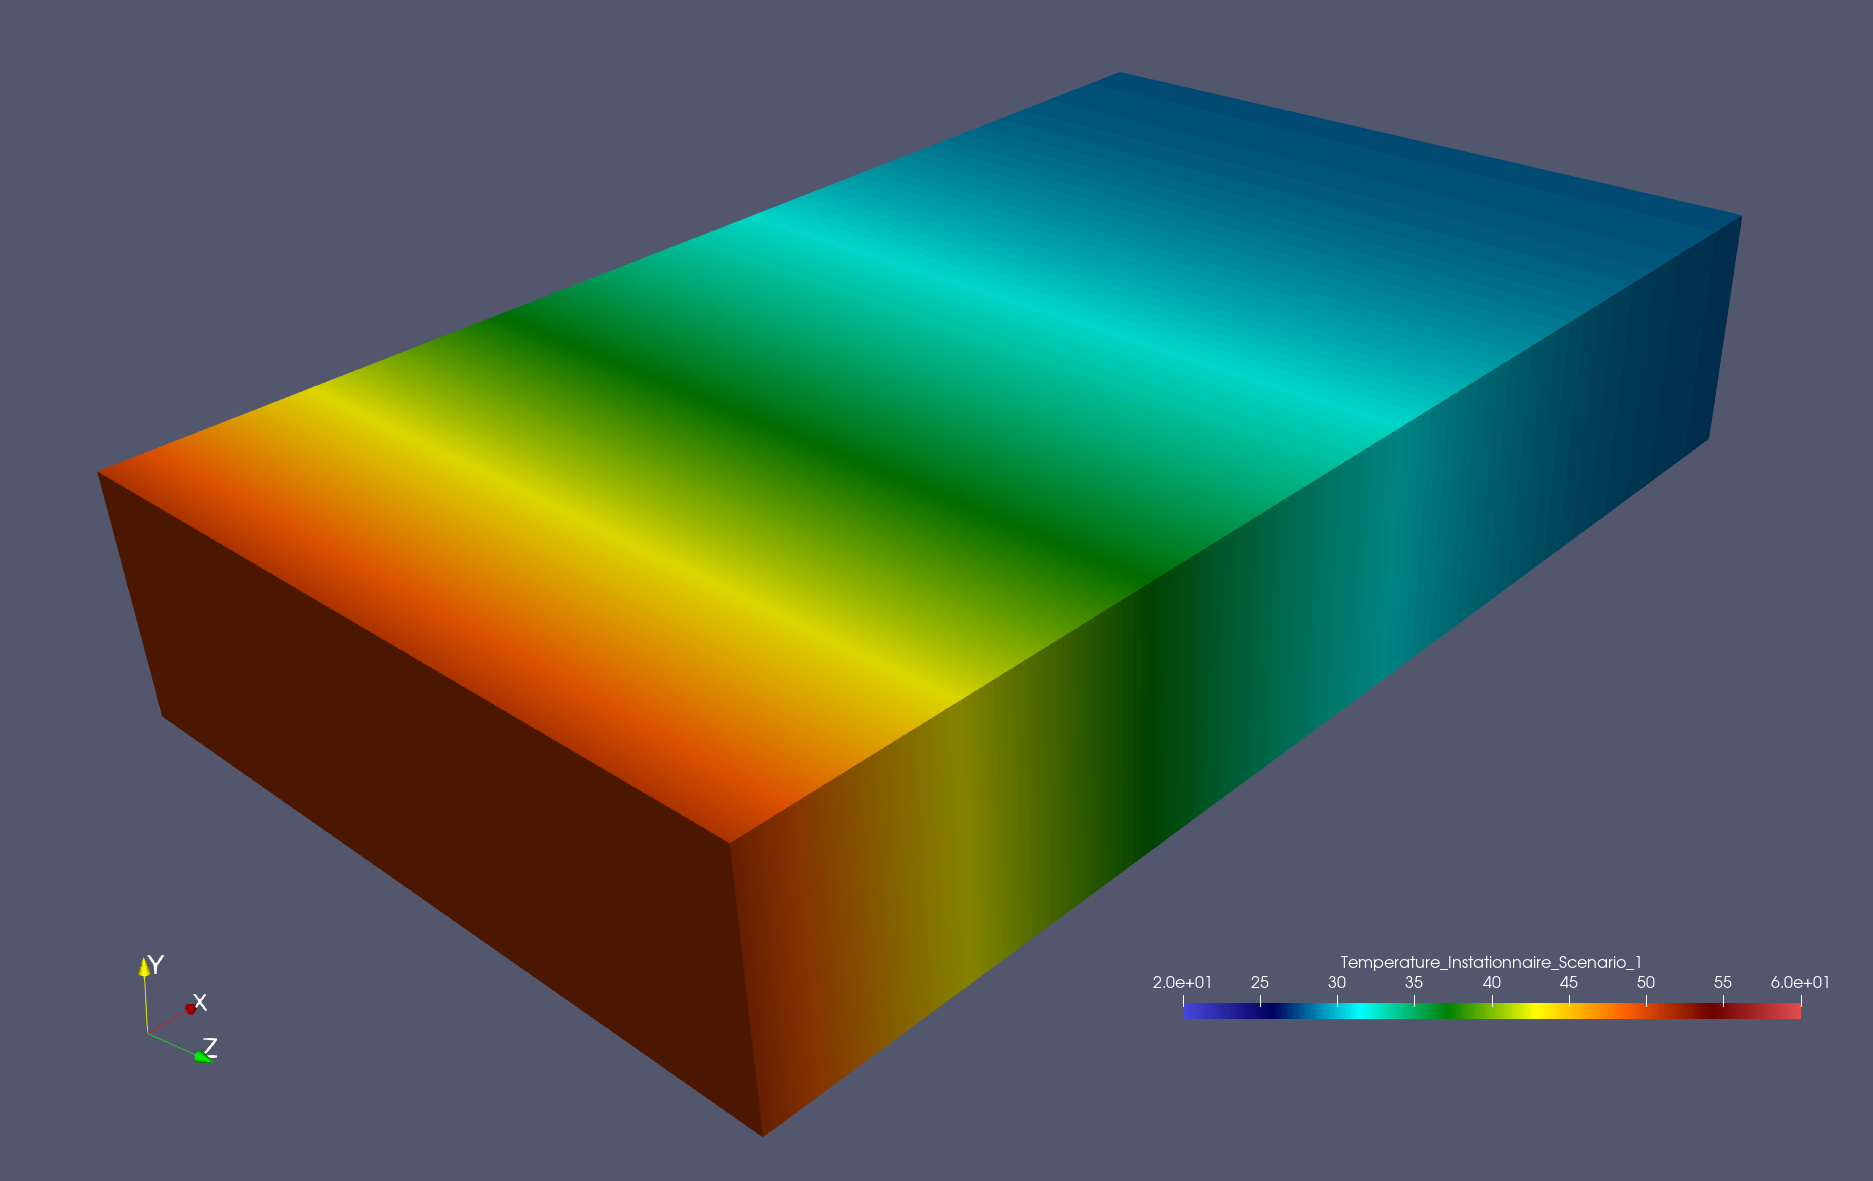
\includegraphics[width=7.5cm]{fig_16} }}%
				\caption{Scénario 1 - Lx = 80 mm}%
			%\end{figure}

			%\begin{figure}[!htb]
				\centering
				\subfloat[Evolution de la température]{{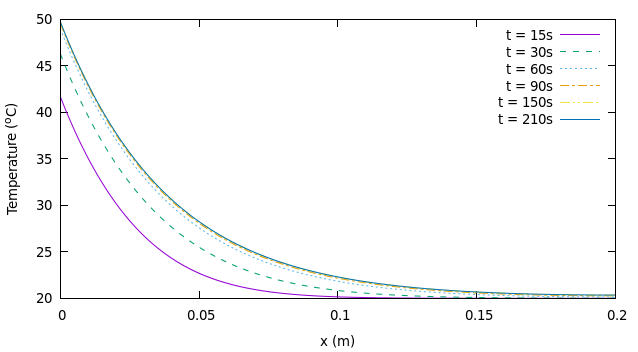
\includegraphics[width=7.5cm]{fig_17} }}%
				\qquad
				\subfloat[Température finale (à t = 300s)]{{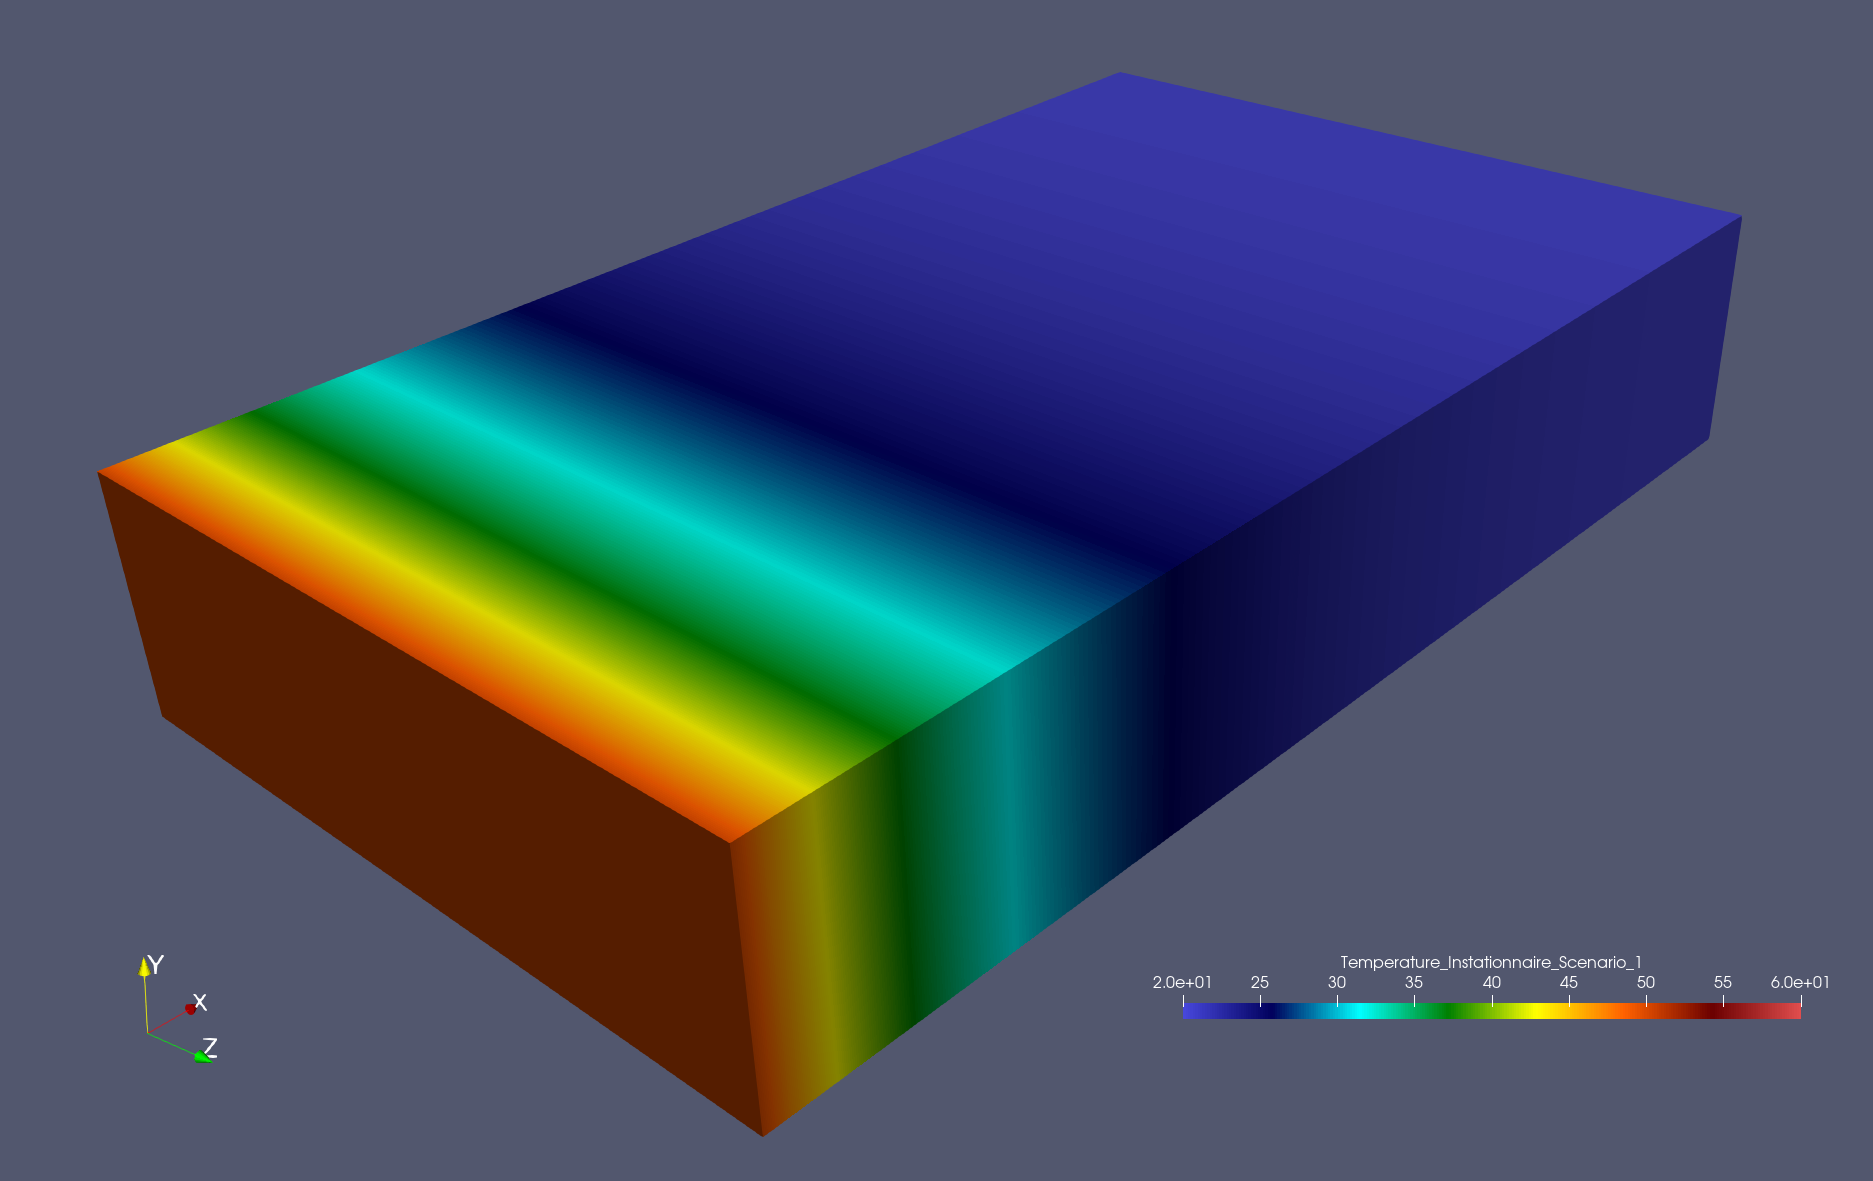
\includegraphics[width=7.5cm]{fig_18} }}%
				\caption{Scénario 1 - Lx = 200 mm}%
			\end{figure}
\par Dans ce cas stationnaire, on remarque que l’évacuation de chaleur est bien meilleure avec des longueurs Lx de plus en plus grandes. En effet, tous les points (et en particulier le point x=0 qui correspond à la température du processeur) sont moins chauds quand Lx augmente.
	
		\begin{center}
			\textbf{Scenario 2: Flux activé et desactivé toutes les 30 secondes}
		\end{center}
\par On utilise ici les fichiers de configuration simu\textunderscore7.cfg, simu\textunderscore8.cfg, et simu\textunderscore9.cfg. La visualisation 3D ici correspond à la température de l’ailette au moment ou le point x=0 est le plus chaud, c’est-à-dire t = 270 s \textbf{(figures 10, 11, et 12)}.
			
			\begin{figure}[!htb]
				\centering
				\subfloat[Evolution de la température en 3 points]{{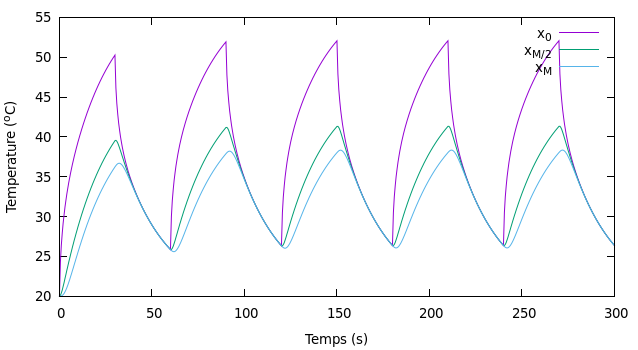
\includegraphics[width=7.5cm]{fig_19} }}%
				\qquad
				\subfloat[Température de l'ailette à l'instant t = 270s]{{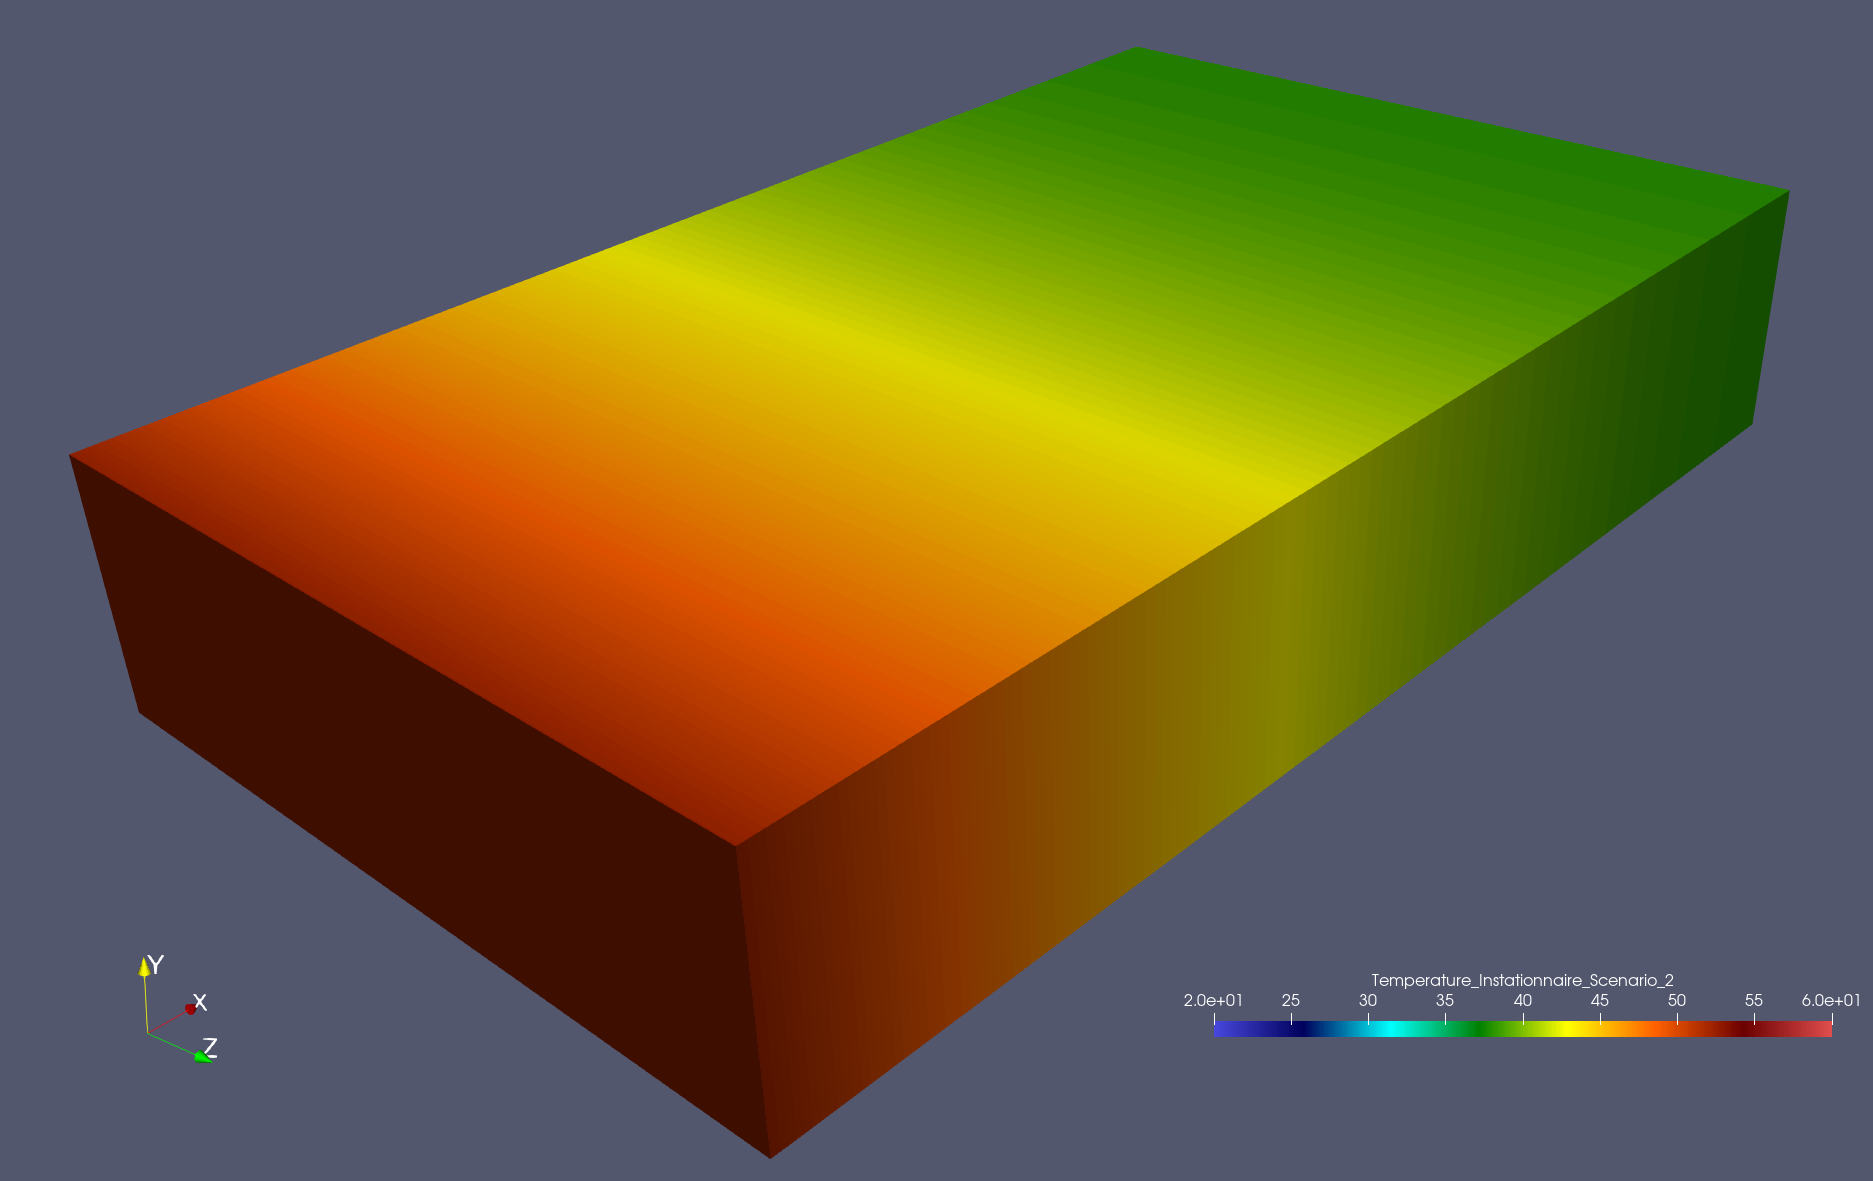
\includegraphics[width=7.5cm]{fig_20} }}%
				\caption{Scénario 2 - Lx = 40 mm}%
			%\end{figure}

			%\begin{figure}[!htb]
				\centering
				\subfloat[Evolution de la température en 3 points]{{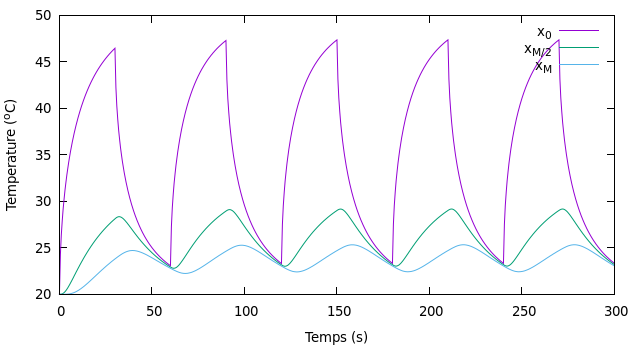
\includegraphics[width=7.5cm]{fig_21} }}%
				\qquad
				\subfloat[Température de l'ailette à l'instant t = 270s]{{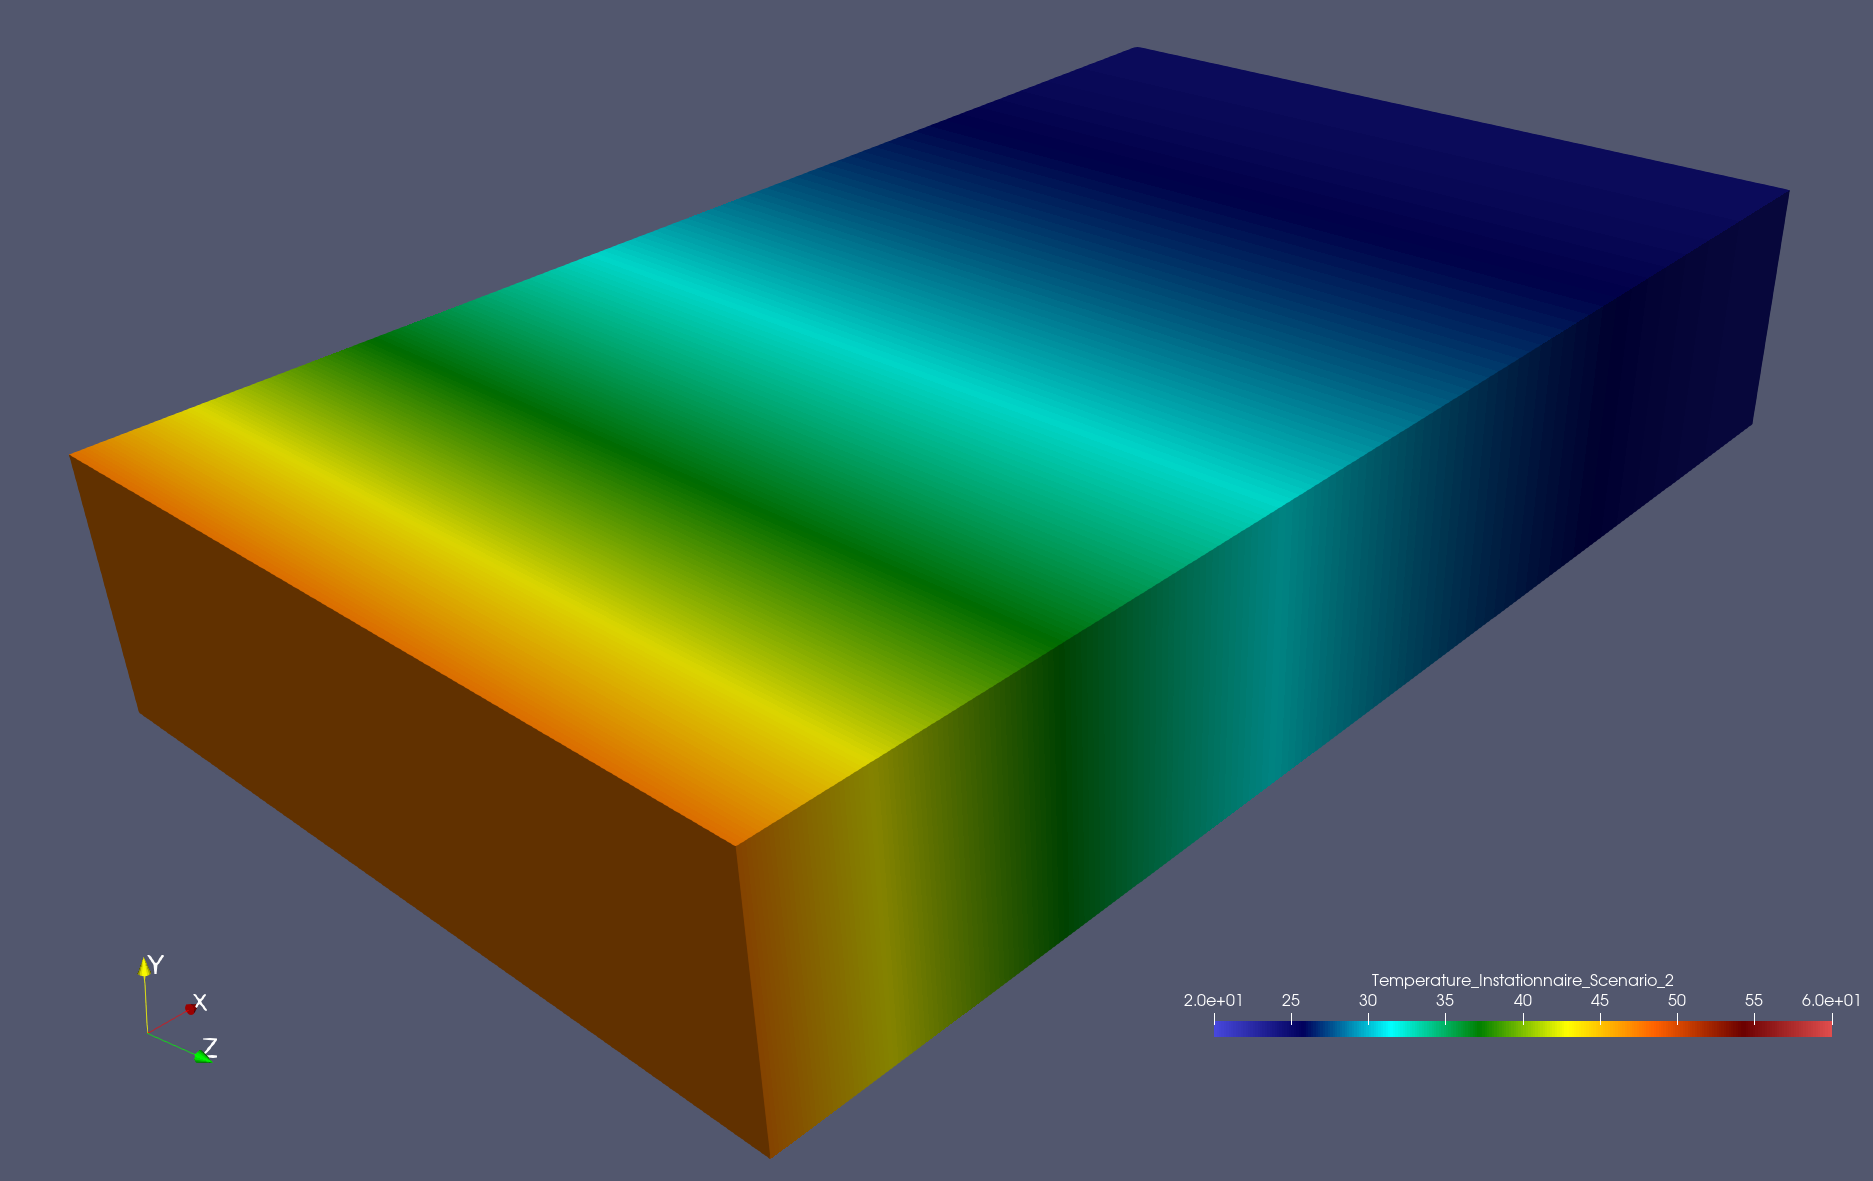
\includegraphics[width=7.5cm]{fig_22} }}%
				\caption{Scénario 2 - Lx = 80 mm}%
			%\end{figure}

			%\begin{figure}[!htb]
				\centering
				\subfloat[Evolution de la température en 3 points]{{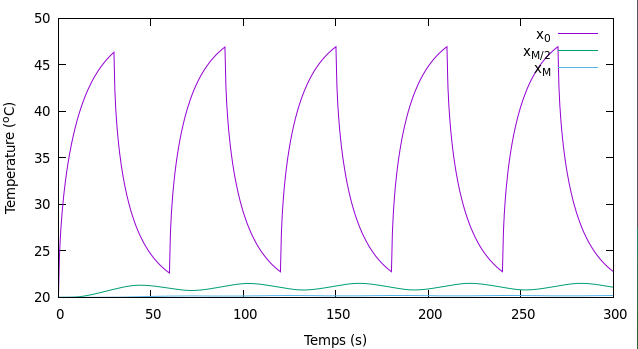
\includegraphics[width=7.5cm]{fig_23} }}%
				\qquad
				\subfloat[Température de l'ailette à l'instant t = 270s]{{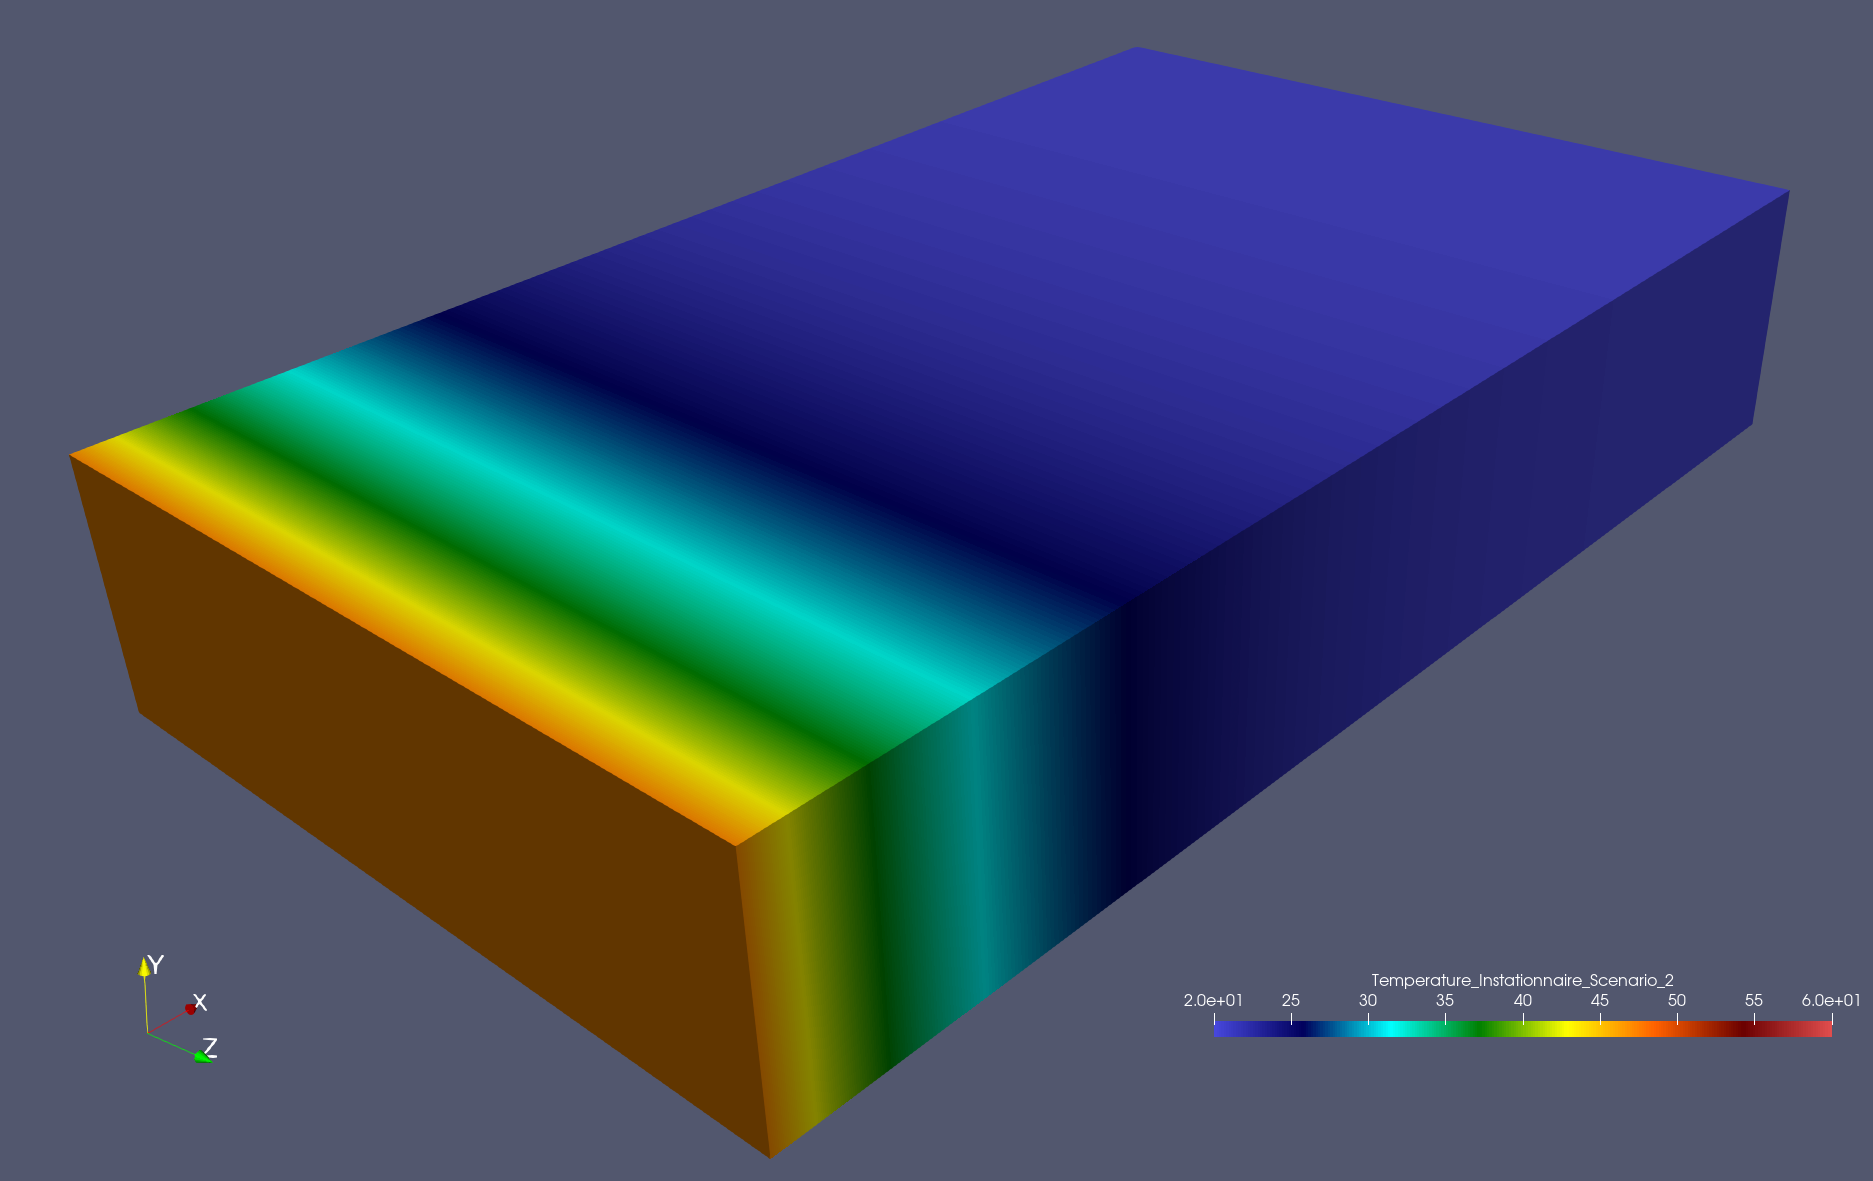
\includegraphics[width=7.5cm]{fig_24} }}%
				\caption{Scénario 2 - Lx = 200 mm}%
			\end{figure}
\par Dans ce scénario, on remarque aussi que la température maximale atteinte par le point le plus chaud du système diminue lorsque Lx augmente. \\
\par En somme, l’augmentation de la longueur Lx améliore de façon considérable l’évacuation de chaleur dans notre dispositif. Ceci est du à l’augmentation de la surface d’échange (par convection) avec l’air ambient qui augmente lorsque L\textsubscript x augmente.
	\subsection{Utilisation ou non du ventilateur}

		\begin{center}
			\bf{Cas 1: Ventilateur allumé (h\textsubscript c = 200 W/(m\textsuperscript2/K))}
		\end{center}
\par Ce scénario correspond aux multiples simulations représentées précédemment. Nous reprenons donc le cas Lx = 40 mm dans le scénario 1 (simu4\textunderscore.cfg, \textbf{figure 13}), et dans le scénario 2(simu\textunderscore7.cfg, \textbf{figure 14}).
			\begin{figure}[!htb]
				\centering
				\subfloat[Evolution de la température]{{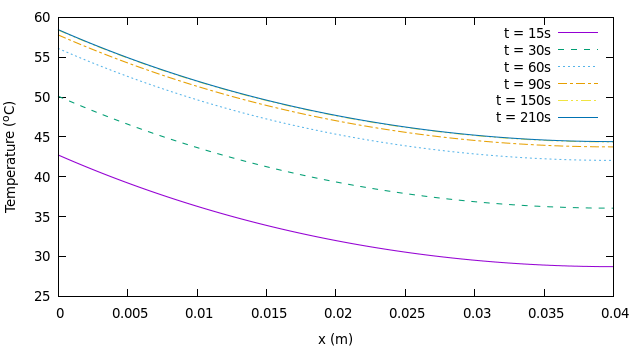
\includegraphics[width=7.5cm]{fig_27} }}%
				\qquad
				\subfloat[Température finale (à t = 300s)]{{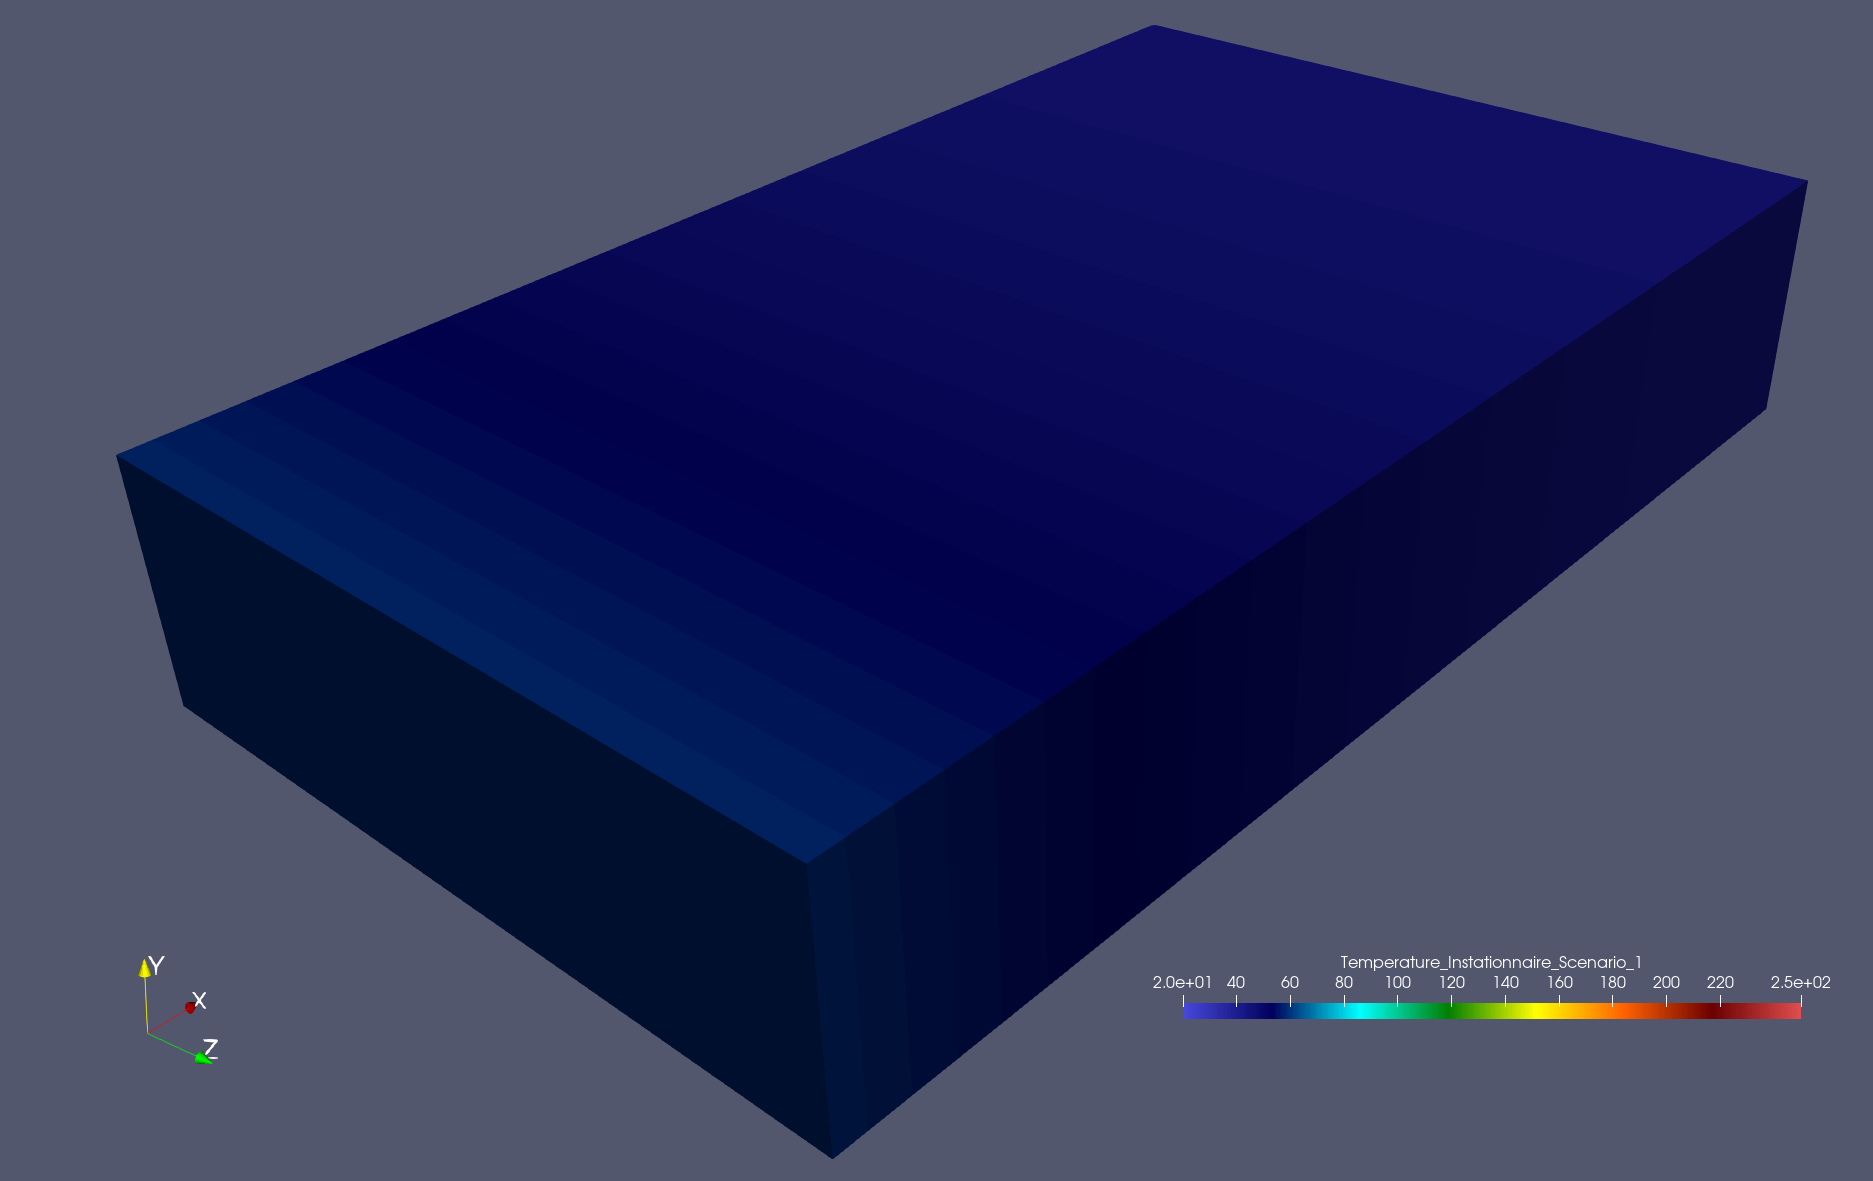
\includegraphics[width=7.5cm]{fig_28} }}%
				\caption{Ventilateur allumé - Scenario 1}%
			%\end{figure}

			%\begin{figure}[!htb]
				\centering
				\subfloat[Evolution de la température pour 3 points]{{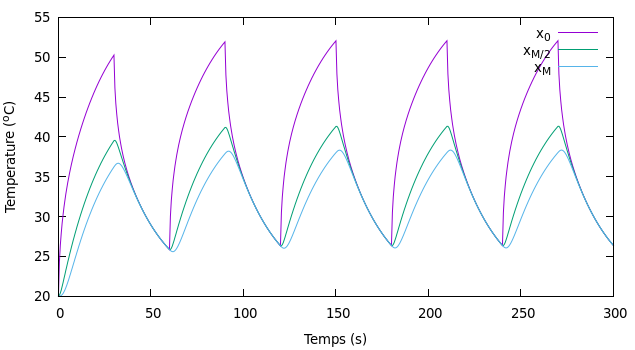
\includegraphics[width=7.5cm]{fig_29} }}%
				\qquad
				\subfloat[Température finale (à t = 300s)]{{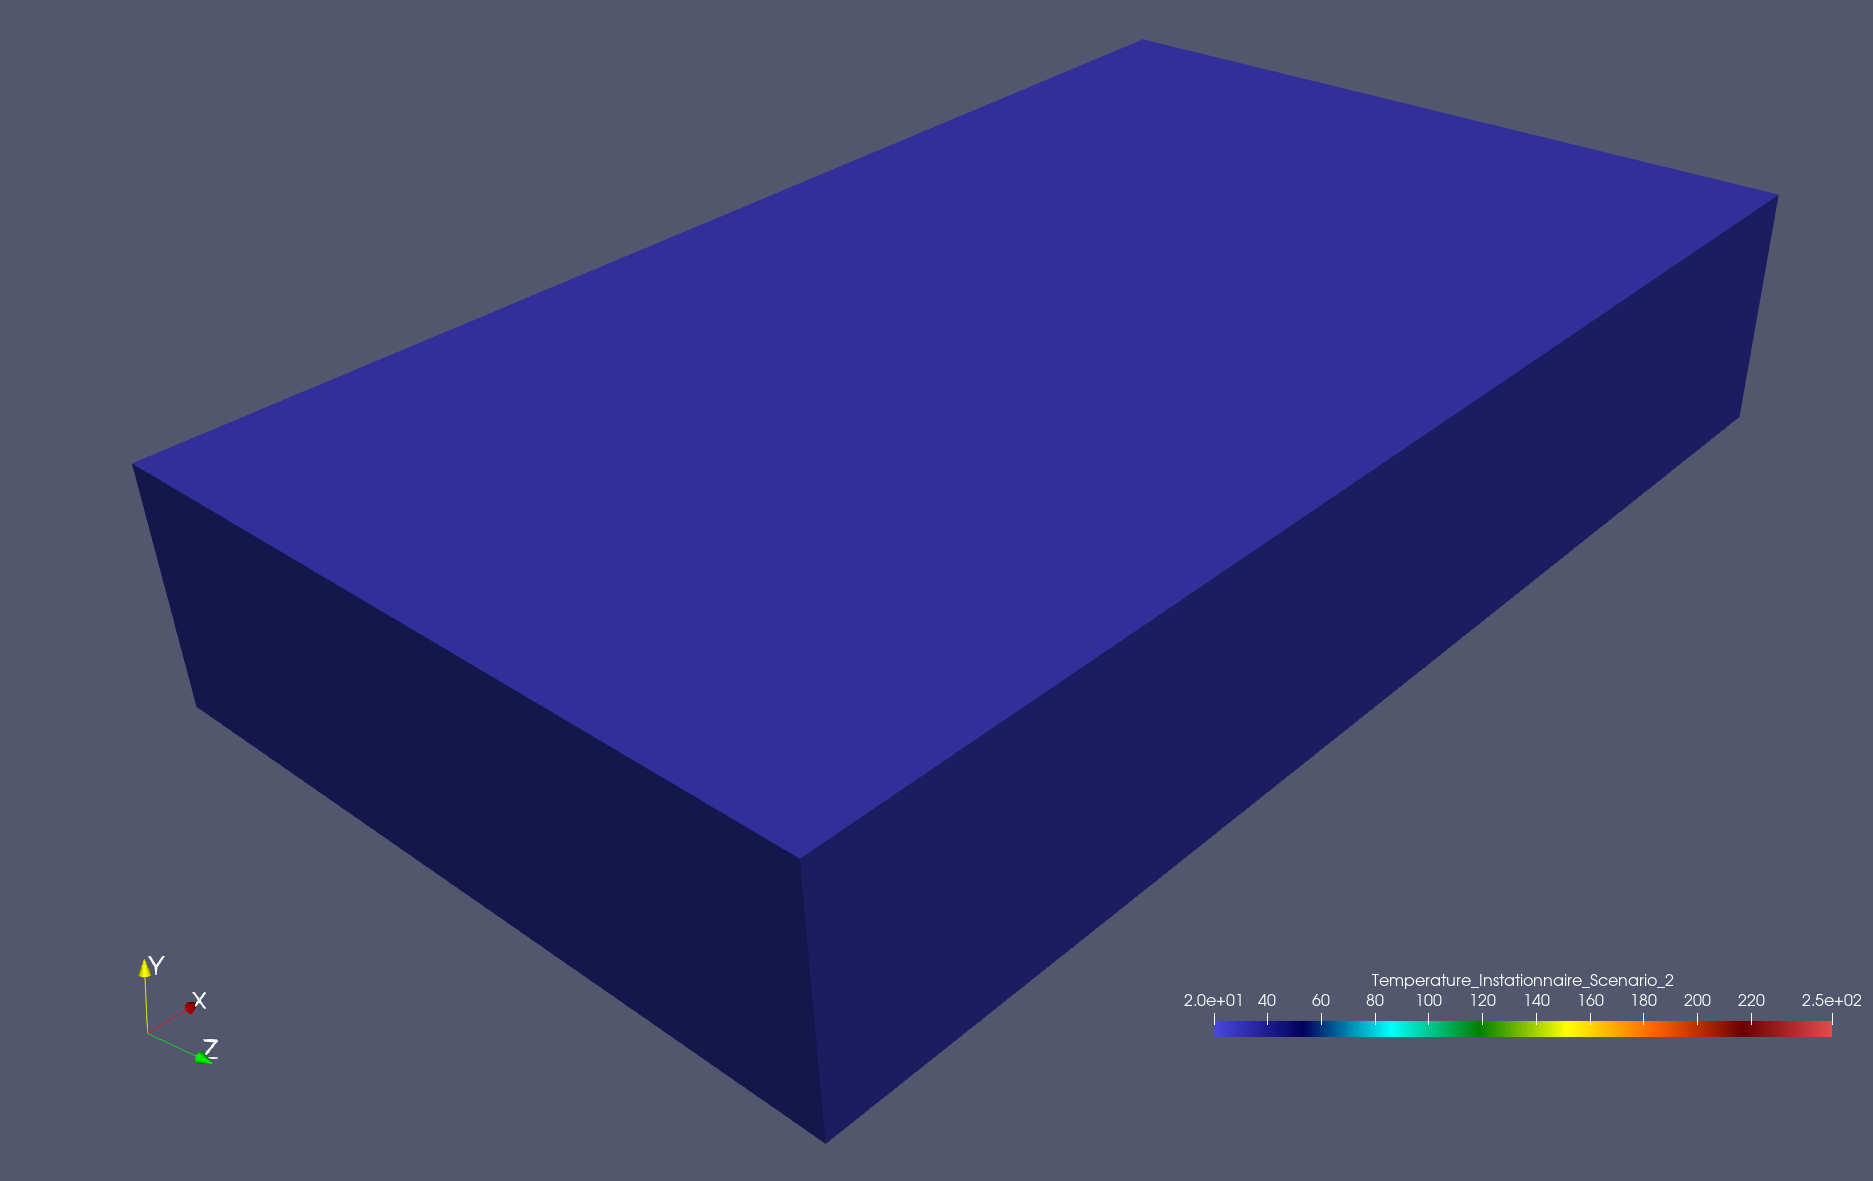
\includegraphics[width=7.5cm]{fig_30} }}%
				\caption{Ventilateur allumé - Scenario 2}%
			\end{figure}

		\begin{center}
			\bf{Cas 2: Ventilateur étteint (h\textsubscript c = 10 W/(m\textsuperscript2/K))}
		\end{center}
\par Nous utilisons ici les fichiers de configuration simu\textunderscore10.cfg (\textbf{figure 15}) et simu\textunderscore11.cfg (\textbf{figure 16}).\\ 
			\begin{figure}[!htb]
				\centering
				\subfloat[Evolution de la température]{{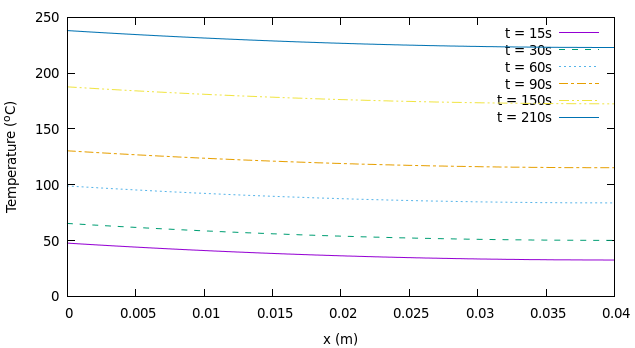
\includegraphics[width=7.5cm]{fig_25} }}%
				\qquad
				\subfloat[Température finale (à t = 300s)]{{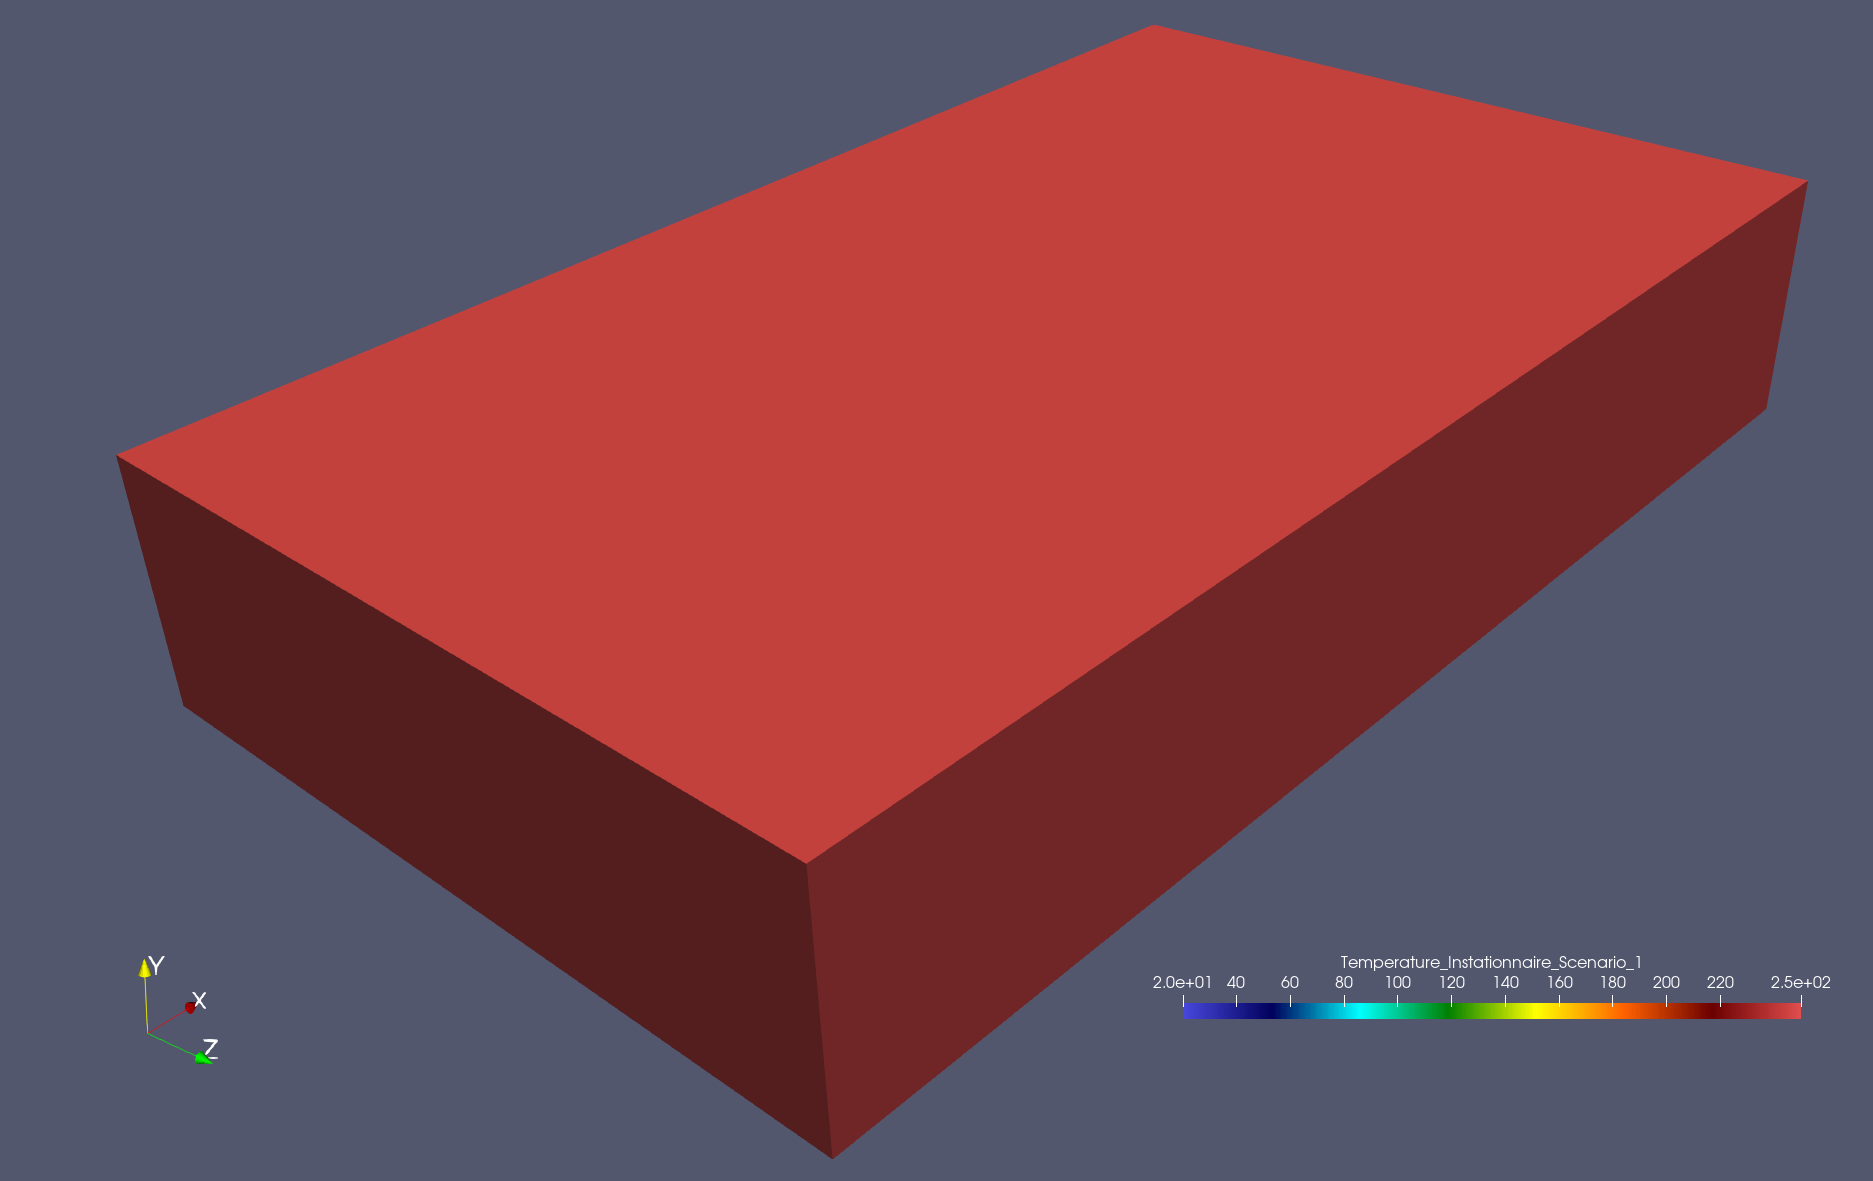
\includegraphics[width=7.5cm]{fig_26} }}%
				\caption{Ventilateur étteint - Scénario 1}%
			%\end{figure}

			%\begin{figure}[!htb]
				\centering
				\subfloat[Evolution de la température pour 3 points]{{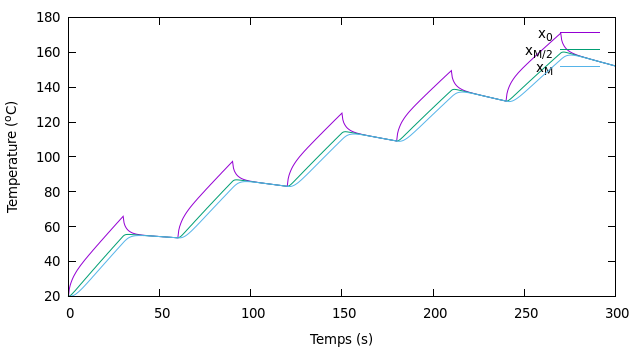
\includegraphics[width=7.5cm]{fig_31} }}%
				\qquad
				\subfloat[Température finale (à t = 300s)]{{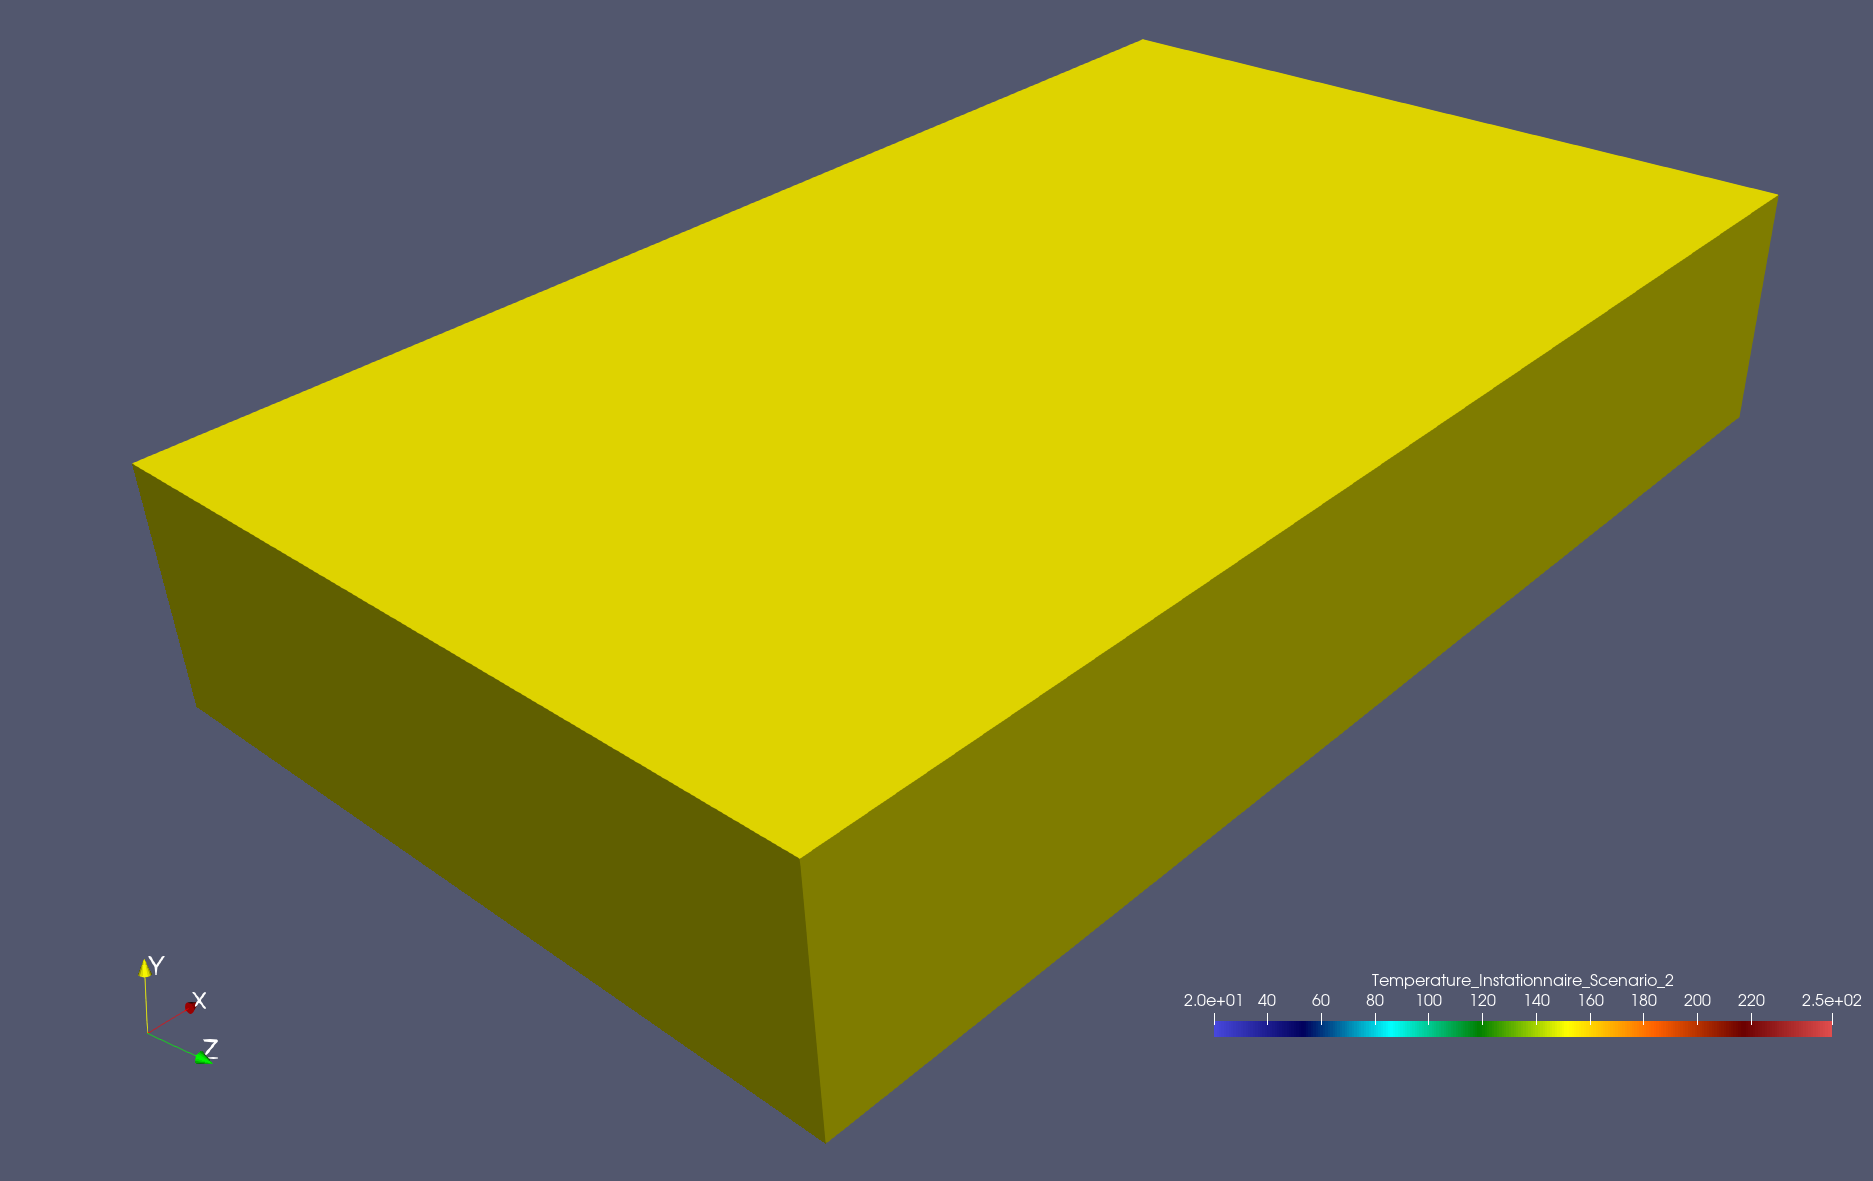
\includegraphics[width=7.5cm]{fig_32} }}%
				\caption{Ventilateur étteint - Scénario 2}%
				\label{fig:conv_stat}%
			\end{figure}
\par Les comparaisons des températures finales (en 3D à droite, sur un intervalle de 20 \degree C à 250 \degree C)  des cas 1 et 2 montre que lorsque le ventilateur est éteint, les températures augmentent grandement sans toutes fois être évacuées. On obtient ainsi une température fulgurante de 250 \degree C lorsque le flux de chaleur venant du processeur est constant (\textbf{figure 15}). Même lorsque le flux de chaleur est activé et désactivé toutes les 30 secondes, on atteint toujours des températures de l’ordre de 180 \degree C sur l’ailette, cela au bout de 300 secondes (\textbf{figure 16}).

\section*{Conclusion}

Le projet a bien permis de simuler le comportement thermique d’une ailette du dissipateur de chaleur. La connaissance de la distribution des températures sur cette ailette nous permet d’imaginer le comportement du système tout entier. On a constaté que le dissipateur doit évacuer des chaleurs très élevées lorsque le ventilateur est éteint, ce qui peut causer son disfonctionnement, peu importe que le flux de chaleur soit activé et désactivé toute les 30s. D’autre part, l’augmentation de la taille du dissipateur (ceci en augmentant la longueur L\textsubscript x de ses ailettes) permet d’assurer une meilleure évacuation de la chaleur. 
\par Le ventilateur a donc une très grande influence sur le système. Il est donc important d’avoir un ventilateur ayant un grand coefficient de transfert surfacique h\textsubscript c pour avoir de bonnes performances du microprocesseur (en vue d’un surcadençage par exemple). Mais cela vient avec un inconvénient majeur qui est que le ventilateur devient très bruyant. On se demande donc si la méthode de refroidissement liquide n’est pas à envisager dans ces cas.


\end{document}
